\documentclass[
 a4paper,
 12pt,
 parskip=half
 ]{scrreprt}
%\setcounter{secnumdepth}{0}
 
\usepackage{settings}

\usepackage{mathpkgs}
\usepackage{mathcmds}

\usepackage[]{fancy_thm}

\usepackage{siunitx}
\sisetup{locale = DE}

\theoremstyle{plain}

\theoremstyle{definition}
%\newtheorem{defn}{Definition}
%\newtheorem{folg}[thm]{Folgerung} 
%\newtheorem{rmrk}[thm]{Bemerkung} 
%\newtheorem{deno}[thm]{Bezeichnungen}
%\newtheorem{exmp}[thm]{Beispiel}
%\newtheorem{aufg}[thm]{Aufgabe} 
%\newtheorem{prgp}[thm]{} % Numbered paragraph

\newtheorem*{rmrk*}{Bemerkung}
%\newtheorem*{exmp*}{Beispiel}
\newtheorem*{defn*}{Definition}
%\newtheorem*{deno*}{Bezeichnungen}

\DeclareMathOperator{\MB}{MB}
\DeclareMathOperator{\BGK}{BGK}

\hypersetup{
  pdftitle={MOSIM},
  pdfauthor={Jonas Hippold},
  hidelinks
}

%opening
\title{Vorlesung\\MoSim - Modellierung und Simulation}
\subtitle{Wintersemester 2017}
\author{Vorlesung: Jun.-Prof. Dr. Christian Mendl\\Mitschrift: Jonas Hippold}

\begin{document}

\maketitle

\tableofcontents

\chapter{Einführung Modellierung und Simulation}
Siehe Folien:

\url{https://tu-dresden.de/mn/math/wir/mendl/ressourcen/dateien/mosim_2017_wise/mosim_2017_intro_slides.pdf}

\chapter{Modellierungsbeispiel: Basketball-Freiwurf}
Trefferquote:
\begin{itemize}
\item Dirk Nowitzki: 89 \%
\item Shaquille O'Neal: 54,4 \%
\end{itemize}
Fragestellung (noch unpräzise): ``Beste Art einen Freiwurf zu werfen?''

Anwendungsproblem: ``Wie sollte ein Basketballspieler einer bestimmten Größe
beim Freiwurf den Ball werfen, damit eine größtmögliche Abweichung beim Abwurf
noch zu einem Treffer führt?''

\section{Erstes Modell: Der beste Abwurfwinkel}
\subsection{Analyse des Anwendungsproblems}
Beobachtung: Nach Verlassen der Wurfhand wird die Flugbahn lediglich durch
physikalische Gesetzmäßigkeiten (Bewegungsgleichungen) bestimmt.
\begin{itemize}
\item Abwurfposition, Anfangsgeschwindigkeit und -richtung, Drehimpuls
\item Luftwiderstand
\item Verschiedene Arten, ins Netz zu gehen
\end{itemize}
$\rightsquigarrow$ ``exakte'' Beschreibung sehr aufwendig bzw. kompliziert.

Vereinfachte Annahmen:
\begin{enumerate}
\item Nur ``nearly nothing but net''-Würfe, entweder direkt ins Netz oder Ball
  trifft Hinterkante des Rings und geht dann ins Netz.
\item Vernachlässigung des Luftwiderstands.
\item Vernachlässigung des Spins.
\item Kein seitlicher Fehler beim Abwurf (2D-Betrachtung statt 3D).
\item Kein Fehler in der Abwurfgeschwindigkeit (zunächst nur Winkel
  untersuchen).
\item Idealer Wurf geht durch das Zentrum des Rings (legt ``ideale''
  Geschwindigkeit fest).
\end{enumerate}

Präzisierte Problemstellung: Mit welchem Abwurfwinkel sollte ein Spieler den
Ball werfen, sodass eine größtmögliche Abweichung vom Winkel immer noch zu einem
Treffer führt?

\subsection{Herleitung eines (ersten) mathematischen Modells}
\subsubsection*{Systemparameter}
(hier Geometrie)

Relevante Maße: (Regelwerk NBA) Foot [\si{ft}], bzw. Inch [\si{in}]
(\SI{1}{in} $=$ \SI{2.54}{\cm}, \SI{1}{ft} $=$ \SI{12}{in} $=$ \SI{0.3048}{\m})
\[ l = \SI{13.5}{ft} = \SI{4.1148}{\m}, \qquad h = \SI{10}{ft} - \frac{5}{4}
  \cdot h_P, \qquad g = \SI{9.807}{\m \per \second \squared}. \]
$h_p$ ... Spielergröße

\subsubsection*{Variablen zur Zustandsbeschreibung}
(Mittelpunkt des Balls)

Ort:
\[ s(t) = \pmat{x(t) \\ y(t)} \in \real^2  \]
wegen Annahme 4.

Geschwindigkeit: $v(t)$ \\
Newtonsche Bewegungsgleichungen (Flugbahn)
\begin{align*}
  v_x(t) &= v_x^0 = \mathrm{const}. \\
  \dot{v}_y(t) &= \diff{}{t} v_y(t) = -g \\
  v_y(t) &= v_y^0 - g \cdot t
\end{align*}

Abwurfwinkel: $\vartheta^0$
\[ \pmat{ v_x^0 \\ v_y^0 } = \pmat{ v^0 \cdot \cos \vartheta^0 \\ v^0 \cdot \sin
    \vartheta^0 } \]
$v^0$: Betrag der Abwurfgeschwindigkeit.

Idealer Wurf durch Zentrum des Rings zum Zeitpunkt $T$:
\[ s(t) = \int_0^t v(\obar{t}) \diffop \obar{t} = \pmat{ v_x^0 t \\ v_y^0 t -
    \rez{2} g t^2 }, \qquad t \ge 0. \]
Forderung:
\begin{align*}
  l &\overset{!}{=} x(T) = v^0 \cdot \cos (\vartheta^0) \cdot T \\
  h &\overset{!}{=} y(T) = v^0 \cdot \sin (\vartheta^0) \cdot T - \rez{2} g T^2
      \tag{$\circ$}
\end{align*}
Die erste Gleichung nach $T$ umstellen, in die zweite einsetzen:
\[  l \cdot \tan(\vartheta^0) - h = \rez{2} g \left( \frac{l}{ v^0
      \cos(\vartheta^0)} \right)^2 \]
und damit folgt
\[  v^0 = \frac{l}{\cos(\vartheta^0)} \sqrt{\frac{g}{2(l \tan(\vartheta^0) -
      h)}}. \]
Eine physikalische Lösung existiert nur für $(l \tan(\vartheta^0) - h) > 0$,
also muss
\[ \arctan \left( \frac{h}{l} \right) < \vartheta^0 < \frac{\pi}{2} \]
gelten.

\subsubsection*{Erlaubte Abweichung vom Abwurfwinkel?}
(bei festgehaltenem $v^0$)

$\tilde{T}$ Zeitpunkt des Erreichens der Höhe $h$, Abwurfwinkel $\vartheta$.
\begin{align*}
  x(\tilde{T}) \tan \vartheta - h
  &= \rez{2} g \left( \frac{x(\tilde{T})}{v^0 \cos \vartheta} \right)^2 \\
  &= \frac{(v^0 \cos \vartheta)^2}{g} \left(
    \tan \vartheta + \sqrt{
    (\tan \vartheta)^2 - \frac{2gh}{(v^0 \cos \vartheta)^2}
    }\right).
\end{align*}
Anmerkung: Auflösen von ($\circ$) liefert
\[ \tilde{T} = \rez{g} \left(
    v_y^0 + \sqrt{(v_y^0)^2 - 2gh}
  \right) \]

\subsubsection*{Rekapitulation}
Bewegungsgleichung:
\[ \pmat{ \ddot{x} \\ \ddot{y} } = \pmat{0 \\ -g } \]
Randbedingung:
\[ \pmat{ x(0) \\ y(0) } = \pmat{ 0 \\ 0 }, \quad \pmat{x(t) \\ y(T)}
  = \pmat{l \\ h}. \]
Flugzeit $T$ ist freier Parameter.

Bedingung für ``Ball geht ins Netz'':
\begin{enumerate}
\item Wurf darf nicht zu lang sein:
  \[ x(\tilde{T}) + R_b \le l + R_r, \]
  $R_b $ ... Radius des Balls, $R_r$ ... Radius des Korbrings.
\item Wurf darf nicht zu kurz sein
  \[ x(\tilde{T}) - R_b \le l - R_r. \]
\item Ball darf Vorderseite des Rings nicht berühren:
  \[ a(t) := \left\| \pmat{x(t) \\ y(t)} - \pmat{l - R_r \\ h} \right\|_2 > R_b. \]
  Anmerkung: Es reicht, das Zeitintervall $[t_0, \tilde{T}]$ mit $t_0 =
  \rez{v_x}(l - R_r - R_b)$ zu überprüfen.
\end{enumerate}

$\vartheta_{\min}$, $\vartheta_{\max}$: Kleinster bzw. größter Winkel, bei dem
der Ball gerade noch in den Korb geht (gegen Referenzwinkel $\vartheta^0$).
\[ e( \vartheta^0 ) := \min \{ v_{\max} - \vartheta^0, \vartheta^0 -
  \vartheta_{\min} \}. \]
Zielfunktional (soll maximiert werden):
\[ \vartheta_{\mathrm{opt}}^0 = \argmax_{\vartheta^0} e( \vartheta^0). \]

Zur Implementierung und Simulation siehe die Python-Beispiele im Netz:\\
\url{https://tu-dresden.de/mn/math/wir/mendl/studium/courses/mosim_2017_wise}

Bis jetzt: Sehr viele Annahmen, um ein relativ einfach zu lösendes Modell zu
erhalten (insbesondere Annahme 5: kein Fehler in der Abwurfgeschwindigkeit).

\section{Zweites Modell: beste Wurfbahn}
\subsubsection*{Beste Wurfbahn}
Annahmen 1, 2, 3 und 4 wie bisher, aber jetzt ohne Annahmen 5 und 6. Variiere
das Tupel $(v^0, \vartheta^0)$ (anstatt $v^0$ fest zu halten).

Problemformulierung: ``Bestimme diejenige Wurfbahn (festgelegt durch $(v^0,
\vartheta^0)$), die die größtmögliche Abweichung erlaubt, sodass der Ball immer
noch in den Korb geht.''

\subsection{Analyse des Anwendungsproblems}
Zu gegebenem $\vartheta^0$ bestimme:
\[ v^0_{\text{front}}, v^0_{\text{back}}, \]
$v^0_{\text{front}}$ ... Ball berührt Korbring vorne (und geht ins Netz), \\
$v^0_{\text{back}}$ ... Ball berührt Korbring hinten (und geht ins Netz).

\subsubsection*{Berechnung von $v^0_{\text{back}}$}
Wir definieren $\bar{T}$ als den Zeitpunkt, zu dem gilt:
\[ x(\bar{T}) = l + R_r - R_b, \qquad y(\bar{T}) = h. \]
Nach analoger Rechnung wie zuvor (mit $x(\bar{T}$ statt $l$) erhalten wir
\[ v^0_{\text{back}} = \frac{l+R_r-R_b}{\cos \vartheta^0}
  \sqrt{\frac{g}{2 ((l + R_r - R_b) \tan \vartheta^0 - h)}}. \]

\subsubsection*{Berechnung von $v^0_{\text{front}}$}
Betrachte $a(t)$: Abstand des Ballmittelpunkts von der Vorderseite des Rings
\[ a_{\min} = \min_{t \in [0, \bar{T}]} \{ a(t) \}, \qquad v^0_{\text{front}}
  := \argmin_{v^0} | a_{\min}(v^0, \vartheta^0) - R_b |. \]
Ball berührt Vorderseite, falls Zielfunktion den Minimalwert 0 erreicht.

Nebenbedingung: $x(\bar{T}) \ge l - R_r$ (Ball fliegt über Vorderseite hinweg).

Berücksichtung der Nebenbedingung im Zielfunktional? Idee: Addiere sie als
``Strafterm'' hinzu.
\[ v^0_{\text{front}}
  := \argmin_{v^0} | a_{\min}(v^0, \vartheta^0) - R_b | + \max \{ 0, l - R_r -
  x(\bar{T})\}. \]
Der Strafterm verschwindet, falls die Nebenbedingung erfüllt wird.

\subsection{Mathematisches Modell: Mehrzieloptimierung}
Relative Abweichungen (sonst nicht vergleichbar)
\[ \begin{aligned}
    e_\vartheta(v^0, \vartheta^0) &:= \min \left(
      \frac{\vartheta_{\max}(\vartheta^0) - \vartheta^0}{\vartheta^0},
      \frac{\vartheta^0 - \vartheta_{\min}(\vartheta^0)}{\vartheta^0}
    \right) \\
    e_v(v^0, \vartheta^0) &:= \min \left(
      \frac{v_{\text{back}}(v^0) - v^0}{v^0},
      \frac{v^0 - v_{\text{front}}(v^0)}{v^0}
    \right)
  \end{aligned} \]

Visualisierung ergibt: Erlaubte Abweichung im Winkel ist größer ($\sim 10
\%$) als erlaubte Abweichung in Geschwindigkeit ($\sim 1 \%$).

Wie sollen $e_\vartheta$ und $e_v$ gleichzeitig optimiert werden?
``Mehrzieloptimierung''
\[ e( v^0, \vartheta^0 ) := \min \{ e_\vartheta(v^0, \vartheta^0), w \cdot
  e_v(v^0, \vartheta^0) \} \]
mit Gewichtungsfaktor $w$.

Mathematisches Optimierungsproblem:
\[ (v^0_{\text{opt}}, \vartheta^0_{\text{opt}}) = \argmax_{(v^0, \vartheta^0)}
  e(v^0, \vartheta^0). \]

\subsubsection*{Auswertung und Interpretation}
Für \SI{2.13}{\m} Spielergröße, $w = 5$:
\[ v^0_{\text{opt}} = \SI{6.7}{\m \per \s}, \qquad \vartheta^0_{\text{opt}} =
  \ang{52.5}. \]

\clearpage

\chapter{Methodik der mathematischen Modellierung}
\section{Modellierungszyklus}
Mathematische Modellierung ist ein iterativer Prozess.

\begin{center}
  \includegraphics{img/modellierung}
\end{center}

Beispiel Basketball-Freiwurf: Zweifaches Durchlaufen des Zyklus.

Analyse des Anwendungsproblems: Beschränkung auf Wurftrajektorie,
vereinfachende Annahmen, Flugbahn nach Abwurf festgelegt durch Bewegungsgleichungen.

Modellbildung: Bewegungsgleichungen, geometrische Bedingungen an Flugbahn.

Mathematisches Modell: Flugbahn
\[ \pmat{x(t)\\y(t)}, \qquad \pmat{v_x(t)\\v_y(t)}. \]
Optimierungsproblem (erstes Modell):
\[ \vartheta_{\mathrm{opt}}^0 = \argmax_{\vartheta^0} e( \vartheta^0). \]

Mathematische Analyse: Zielfunktional $e(\vartheta^0)$ ist nicht stetig
differenzierbar $\rightsquigarrow$ Optimierung ohne Verwendung von Gradienten.

Interpretation und Validierung: Vergleich mit experimentellen Daten.

\section{Mathematisches Modell}
\begin{defn*}
  Ein \emph{mathematisches Modell} stellt formale Zusammenhänge zwischen
  (physikalischen bzw. Modell-) Größen her. Eine solche Größe ist eine
  quantitative Eigenschaft eines physikalischen Objektes, Zustands oder
  Prozesses. Man unterscheidet zwischen Parametern und Variablen.

  Aus der Analyse bzw. Simulation eines mathematischen Modells sollen
  Erkenntnisse über das reale (physikalische) System gewonnen werden.
\end{defn*}

\subsubsection*{Parameter}
\begin{itemize}
\item Systemparameter (z.B. Korbhöhe beim Basketball-Freiwurf)
\item Modellparameter (z.B. Schrittweite beim diskreten Modell)
\end{itemize}

\subsubsection*{(Zustands-) Variablen} (z.B. Trajektorie $\pmat{x(t)\\y(t)}$,
$\pmat{v_x(t)\\v_y(t)}$) bei Berücksichtung der Drehung eines (starren) Körpers
zusätzlich Rotation, beschrieben typischerweise durch Quaternionen)

\subsubsection*{Mathematische Analyse eines Modells}
\begin{itemize}
\item Dimensionsanalyse und Skalierung
\item Existenz und Eindeutigkeit einer Lösung
\item Untersuchung von Sonderfällen
\item Falls explizite Lösung angegeben werden kann: Validierung der numerischen
  Lösung
\item Vereinfachung, Linearisierung; Störungstheorie
\item Untersuchung von qualitativen Eigenschaften, etwa asymptotisches Verhalten
\item Sensitivitätsanalyse: Wie wirken sich Störungen von Parametern auf die
  Lösung aus?
\item Auswahl von numerischen Verfahren
\end{itemize}

\section{Dimensionsanalyse und Skalierung}
Größe $X$, Dimension $[X]$, z.B:
\[ [l] = \text{Länge}, \qquad [t] = \text{Zeit}, \qquad [v] =
  \text{Geschwindigkeit} = \frac{\text{Länge}}{\text{Zeit}}. \]

Iternationales Einheitensystem SI

\subsubsection*{Basiseinheiten}
\begin{center}
  \begin{tabular}{l|c|c|c|c}
    Dimensionsname & Größensymbol & Dimensionssymbol & Einheit & Zeichen \\
    \hline
    Länge & $l$ & $L$ & Meter & \si{\m} \\
    Masse & $m$ & $M$ & Kilogramm & \si{\kg} \\
    Zeit  & $t$ & $T$ & Sekunde & \si{\s} \\
    Stromstärke & $I$ & $I$ & Ampere & \si{\ampere} \\
    Temperatur & $T$ & $\Theta$ & Kelven & \si{\kelvin} \\
    Stoffmenge & $n$ & $N$ & Mol & \si{\mol} \\
    Lichtstärke & $Ir$ & $J$ & Candela & \si{\candela}
  \end{tabular}
\end{center}

Abgeleitete Größen und Einheiten, zum Beispiel:
\begin{center}
  \begin{tabular}{l|c|c|c|c}
    Geschwindigkeit & $v$ & $\frac{L}{T}$
    & $\frac{\text{Meter}}{\text{Sekunde}}$ & \si{\m \per \s} \\
    Kraft & $F$ & $M \cdot \frac{L}{T^2}$
    & Newton & $\si{\newton} = \si{\kg \m \per \s \squared}$ \\
    Energie/Arbeit & $E$ & $M \cdot \frac{L^2}{T^2}$
    & Joule & $\si{\joule} = \si{\newton \m} = \si{\kg \m \squared \per \second \squared}$ \\
    Leistung & $P$ & $M \cdot \frac{L^2}{T^3}$
    & Watt & $\si{\joule \per \s} = \si{\kg \m \squared \per \second \cubed}$ \\
    Elektrische Leistung & $Q$ & $J \cdot T$
    & Couloumb & $\si{\coulomb} = \si{\ampere \s}$
  \end{tabular}
\end{center}

Grundlegende Eigenschaften und Regeln:
\begin{itemize}
\item Multiplikation, Potenzieren, Division von dimensionsbehafteten Größen
  überträgt sich auf Dimensionen.

  Beispiel: \\
  Volumen eines Kubus
  \[ V = (\text{Kantenlänge } a)^3, \qquad [V] = L^3. \]
  Geschwindigkeit
  \[ \left[ \diff{}{t} x(t) \right] = \left[ \lim_{\Delta t \to 0} \frac{x(t +
        \Delta t) - x(t)}{\Delta t} \right] = \frac{L}{T}. \]
  Beschleunigung
  \[ \left[ \frac{\diffop^2}{\diffop t^2} x(t) \right] = \frac{L}{T^2}. \]
\item Nur Größen gleicher Dimension dürfen addiert, subtrahiert und verglichen
  werden.

  Beispiel: Zweites Newtonsches Gesetz, ``Kraft $=$ zeitliche Änderung des
  Impulses''
  \[ F = \diff{}{t} p(t), \qquad p = m \cdot v, \]
  \[ [ F ] = \frac{[p]}{[t]} = \frac{M \cdot L/T}{T} = M \cdot \frac{L}{T^2}. \]
\item Argumente von Funktionen\footnote{%
    Ausnahme: Monome. Das sind Polynome, die nur aus einem Glied bestehen. Ein
    Monom ist ein Produkt, bestehend aus einem Koeffizienten und einer Potenz
    einer Variablen.}%
  müssen dimensionslos sein. Zum Beispiel ist $\exp(x)$ mit $[x] = L$
  \emph{nicht} zulässig, da
  \[ \exp(x) = 1 + x + \rez{2} x^2 + \rez{6} x^3 + \ldots, \]
  das ergibt keinen Sinn. Zulässig ist aber
  \[ \exp( k \cdot x ) \qquad \text{mit} \qquad [k] = \rez{L}, [x] = L. \]
  Dann ist $k \cdot x$ wieder dimensionslos.
  \[ F(t) = F_0 \cdot \sin (\omega t), \quad [t] = T, \quad [\omega] =
    \rez{T}. \]
\end{itemize}

\section{Entdimensionalisierung}
Beobachtung:  Mathematische Aussagen über ein mathematisches (physikalisches)
Modell können nicht von der Wahl der Einheiten der jeweiligen Größen abhängen.
$\rightsquigarrow$ Transformation auf eine dimensionslose Form.

Beispiel: senkrechter Wurf, Gravitationskraft auf einen geworfenen Ball.
Gravitationsgesetz: 
\[ F = \gamma \frac{ m_1 m_2 }{ r^2 }. \]
$\gamma = \SI{6.674e-3}{\m \cubed \per \kg \per \s \squared}$ ...
Gravitationskonstante. $[\gamma] = \frac{L^3}{MT^2}$.

Berücksichtige den Erdradius $R$:
\[ F = - \gamma \frac{ m \cdot m_E }{ (x(t) + R)^2 } \]
Anwendung des zweiten Newtonschen Gesetzes:
\begin{align*}
  \diff{}{t} \underbrace{m \dot{x}(t)}_{\text{Impuls}} &= F \\
  m \ddot{x}(t) &= - \gamma \frac{ m \cdot m_E }{ (x(t) + R)^2 }
\end{align*}
Speziell für die Erde:
\[ R = \SI{6371}{\km}, \qquad m_E = \SI{5.9722e24}{\kg}, \qquad g = \frac{\gamma
    \cdot m_E}{R^2} = \SI{9.81}{\m \per \second \squared} \]
Einsetzen:
\[ \ddot{x}(t) = -g \frac{R^2}{(x(t) + R)^2} \]

Anfangsbedingungen $x(0) = 0$, $\dot{x}(0) = \bar{v}$.

\subsubsection*{Entdimensionalisierung}
Referenzlänge $\ell_0$, $[\ell_0] = L$ \\
Referenzzeit $\tau_0$, $[\tau_0] = T$ \\
Neue dimensionslose Variablen:
\[ \hat{x} = \frac{x}{\ell_0}, \qquad \hat{t} = \frac{t}{\tau_0} \qRq
  \hat{x}(\hat{t}) = \rez{\ell_0} x ( \tau_0 \hat{t} ). \]
Also folgt
\[ \diff{}{\hat{t}} \hat{x}(\hat{t})
  = \frac{\tau_0}{\ell_0} \dot{x}(\tau_0 \hat{t}), \qquad
  \frac{\diffop^2}{\diffop \hat{t}^2} \hat{x}(\hat{t}) = \frac{\tau_0^2}{\ell_0}
  \ddot{x}( \tau_0 \hat{t}). \]
Einsetzen:
\[ \frac{\diffop^2}{\diffop \hat{t}^2} \hat{x}(\hat{t}) =
  - \frac{\tau_0^2}{\ell_0} g \rez{\left( \frac{\ell_0}{R} \hat{x}(\hat{t}) + 1
    \right)^2}. \]
Anfangsbedingungen $\hat{x}(0) = 0$, $\diff{}{\hat{t}}\hat{x}(0) =
\frac{\tau_0}{\ell_0} \bar{v}$.

Wir bezeichnen:
\[ \Pi_1 := \frac{\tau_0^2}{\ell_0} g, \qquad
  \Pi_2 := \frac{\ell_0}{R}, \qquad
  \Pi_3 := \frac{\tau_0}{\ell_0} \bar{v}. \]
$\Pi_1$, $\Pi_2$ und $\Pi_3$ sind drei Gruppen von Parametern. Wir können
$\ell_0$ und $\tau_0$ so wählen, dass zwei der drei $\Pi$-Terme gleich 1 sind.

Beobachtung: Für realistische Wurfhöhe $h \ll R$ gilt $\Pi_2 \ll 1$
\[ \left. \begin{aligned}
      \Pi_1 &= 1: & \ell_0 &= g \cdot \tau_0^2 \\
      \Pi_2 &= 1: & \ell_0 &= \bar{v} \tau_0
    \end{aligned}
  \right\} \quad \tau_0 = \frac{\bar{v}}{g}, \quad \ell_0 =
  \frac{\bar{v}^2}{g}. \]
Also gilt
\[ \Pi_3 = \frac{\bar{v}}{gR} =: \eps. \]
Einsetzen:
\[ \frac{\diffop^2}{\diffop \hat{t}^2} \hat{x}(\hat{t}) = - \rez{(\eps
    \hat{x}(\hat{t}) + 1)^2} \]
mit $\hat{x}(0) = 0$, $\diff{}{\hat{t}} \hat{x}(0) = 1$.

Die näherungsweise Lösung für $\eps = 0$ ist
\[ \frac{\diffop^2}{\diffop \hat{t}^2} \hat{x}(\hat{t}) \approx -1, \]
das heißt wir erhalten die ``übliche'' Bewegungsgleichung
\[ \ddot{x}(t) = - g. \]

\subsubsection*{Systematisches Vorgehen}
Zur Bestimmung der Referenzgrößen in komplizierteren Systemen ist es
nicht immer möglich, wie oben intuitiv die richtigen Größen zu bestimmen. Formal
geht man daher wie folgt vor:
\[ \ddot{x}(t) = - g \frac{R^2}{(x(t) + R)^2}, \]
Anfangsbedingungen $x(0) = 0$, $\dot{x}(0) = \bar{v}$.

\begin{enumerate}
\item Unabhängige Dimensionen: Länge $L$, Zeit $T$.
\item Variablen und Parameter: \\
  Variablen: $x$, $[x] = L$; $t$, $[t] = T$.
  Parameter: $\bar{v}$ ($LT^{-1}$), $g$ ($LT^{-2}$), $R$ ($L$).
\item Dimensionslose Größen:
  Ansatz
  \[ \left[ \bar{v}^{\alpha_1} \cdot g^{\alpha_2} \cdot R^{\alpha_3} \right] =
    1. \]
  Also
  \[ \left( \frac{L}{T} \right)^{\alpha_1} \cdot
    \left( \frac{L}{T^2} \right)^{\alpha_2} \cdot
    L^{\alpha_3} = 1 \qRq L^{\alpha_1 + \alpha_2 + \alpha_3} \cdot T^{- \alpha_1
      - 2 \alpha_2} = 1. \]
  Ausgedrückt als lineares Gleichungssystem
  \begin{center}
  \begin{tabular}{l|ccc}
    & $\bar{v}$ & $g$ & $R$ \\
    \hline
    L & 1 & 1 & 1 \\
    T & -1 & -2 & 0
  \end{tabular}
  $\Rightarrow$
  $S = \pmat{ 1 & 1 & 1 \\ -1 & -2 & 0}$.
  \end{center}
  \[ S \alpha = \pmat{ 1 & 1 & 1 \\ -1 & -2 & 0} \pmat{ \alpha_1 \\ \alpha_2 \\
      \alpha_3} = \pmat{0\\0} \]
  Allerdings gilt $\dim \ker S = 3 - 2 = 1$,
  \[ \ker S = \spn \left\{ \pmat{ 2 \\ -1 \\ -1} \right \}. \]

  $\bar{v}^2 g^{-1} R^{-1} =: \eps$ ist dimensionslos (i.A. können mehrere
  ``entdimensionalisierte'' Parameter auftreten).
\item Referenzgrößen:
  \[ \hat{x} = \frac{x}{\ell_0}, \qquad \hat{t} = \frac{t}{\tau_0}. \]
  Ansatz:
  \[ \ell_0 = \bar{v}^{\alpha_1} g^{\alpha_2} R^{\alpha_3}, \]
  Gleichheit der Dimensionen erfordert
  \[ S \alpha = \pmat{1 \\ 0} \qRq \alpha = c \cdot \pmat{2 \\ -1 \\ -1} +
    \pmat{0 \\ 0 \\ 1} \]
  (Lösung nicht eindeutig!). Also folgt
  \[ \ell_0 = R \cdot \eps^c, \]
  im Beispiel oben galt $c = 1$, also $\ell_0 = \frac{\bar{v}^2}{g}$.

  Analog für die Referenzzeit:
  \[ \tau_0 = \bar{v}^{\alpha_1} g^{\alpha_2} R^{\alpha_3}, \qquad S \alpha =
    \pmat{0 \\ 1}. \]
  Also folgt
  \[ \alpha = c' \pmat{2 \\ -1 \\ -1} + \pmat{1 \\ -1 \\ 0 } \]
  und damit $\tau_0 = \frac{\bar{v}}{g} \eps^{c'}$, im Beispiel oben $c' = 0$,
  $\tau_0 = \frac{\bar{v}}{g}$.
\item Aufstellen der entdimensionalisierten Modellgleichung (selbe Rechnung wie
  oben)
  \[ \ddot{\hat{x}}( \hat{t} ) = -\rez{(\eps \hat{x}(\hat{t}) + 1)^2}, \qquad
    \hat{x}(0) = 0, \qquad \dot{\hat{x}}(0) = 1. \]
\end{enumerate}

\begin{rmrk*}
  Für die Wahl $\ell_0 = R$ und $\tau_0 = \frac{\bar{v}}{g}$ erhält man
  \[ \ddot{\hat{x}}(\hat{t}) = - \eps \rez{(\hat{x}(\hat{t}) + 1)^2}, \qquad
    \hat{x}(0) = 0, \qquad \dot{\hat{x}}(0) = \eps. \]
  Das ist mathematisch korrekt, aber wir erhalten keine Näherungslösung für
  $\eps \approx 0$.
\end{rmrk*}

Mit dem obigen Verfahren haben wir die Anzahl der freien Parameter von drei
(Gravitationskonstante, Erdradius, Erdmasse) auf eins ($\eps$) reduziert. Im
Allgemeinen lässt sich immer die Anzahl der Parameter um die Anzahl der
vorhandenen Dimensionen (hier Länge, Zeit) reduzieren.

\begin{thm}[Buckinghamsches $\Pi$-Theorem]
  Gegeben sei ein mathematisches Modell mit $k$ Variablen $x_1, \ldots, x_k$ und
  $l$ Parametern $x_{k+1}, \ldots, x_{k+l}$, in dem $m$ unabhängige Dimensionen
  vorkommen. Dann können $k + l - m$ dimensionslose Größen $q_1, \ldots,
  q_{k+l-m}$ als Produkte und Quotienten von $x_1, \ldots, x_{k+l}$ definiert
  werden und jede skalare Modellgleichung $f(x_1, \ldots, x_{k+l}) = 0$ kann auf
  eine Relation $\hat{f}( q_1, \ldots, q_{k+l-m} ) = 0$ reduziert werden.
\end{thm}

Für unser Beispiel: $m = 2$
\begin{align*}
  f( x, t, \bar{v}, g, R) = 0 \qquad
  &\left\{ \begin{aligned}
      \ddot{x}(t) = -g \frac{R^2}{(x(t) + R)^2} \\
      x(0) = 0, \dot{x}(0) = \bar{v}
    \end{aligned}
  \right. \\ 
  \rightsquigarrow \qquad
  f( \hat{x}, \hat{t}, \eps) = 0 \qquad
  &\left\{ \begin{aligned}
      \ddot{\hat{x}}(\hat{t}) = - \rez{(\eps \hat{x}(\hat{t}) + 1)^2} \\
      \hat{x}(0) = 0, \dot{\hat{x}}(0) = 1
    \end{aligned}
  \right.
\end{align*}

Konsequenz: Aussagen über das Modell, ohne Modellgleichungen zu kennen!

Beispiel Pendel. Schwingungsdauer $t_{sd}$?

Vorwissen/Intuition: Für kleine Auslenkungen ($\vartheta \ll 1$) sollte $t_{sd}$
nicht von den Anfangsbedingungen abhängen (Auslenkung, Geschwindigkeit). Es
sollte eine Relation zwischen $t_{sd}$ und den Parametern $l$, $m$ und $g$ der
Form
\[ f( t_{sd}, g, m, l ) = 0 \]
existieren. Also haben wir $m=3$ unabhängige Dimensionen $T, L, M$.

Buckinghamsches $\Pi$-Theorem $\rightsquigarrow$ Reduktion auf $\hat{f}(q) = 0$
mit der dimensionlosen Größe
\[ q = t_{sd}^{\alpha_1} \cdot l^{\alpha_2} \cdot m^{\alpha_3} \cdot
  g^{\alpha_4} \]
Dimensionsanalyse:
\begin{center}
  \begin{tabular}{r|cccc}
    & $t_{sd}$ & $l$ & $m$ & $g$ \\
    \hline
    $T$ & 1 & 0 & 0 & -2 \\
    $L$ & 0 & 1 & 0 & 1 \\
    $M$ & 0 & 0 & 1 & 0
  \end{tabular}
\end{center}
$q$ muss dimensionslos sein, also:
\[ S\alpha = 0 \qRq \alpha = c \pmat{1 \\ -1/2 \\ 0 \\ 1/2 } \]
und damit
\[ q = t_{sd} l^{-1/2} m^0 g^{1/2}, \qquad t_{sd} = q \sqrt{\frac{l}{g}}. \]
Die Schwingungsdauer ist unabhängig von $m$! Diese Aussage ist ohne Kenntnis der
genauen Systemgleichungen möglich.

Insbesondere ändert eine Skalierung $l \to s \cdot l$, $g \to s \cdot g$ die
Schwingungsdauer nicht.

Bemerkung: Die tatsächliche Lösung ist $t_{sd} = 2 \pi \sqrt{l/g}$.

%%% Local Variables:
%%% TeX-master: "master"
%%% End:

\clearpage

\chapter{Strömungssimulation mit der Lattice-Boltzmann-Methode}
\section{Kinetische Theorie und Boltzmann-Gleichung}
\begin{itemize}
\item $N$ Teilchen (Atome, Moleküle, ...) mit den Größen
\item  $\vec{x}_i \in \real^3$ ... Position des $i$-ten Teilchens,
\item $\vec{p}_i \in \real^3$ ... Impuls des $i$-ten Teilchens.
\end{itemize}

Mikroskopische Bewegungsgleichungen
\begin{equation}
 \diff{\vec{x}_i}{t} = \pdiff{H}{\vec{p_i}}, \qquad \diff{\vec{p}_i}{t} = -
  \pdiff{H}{\vec{x}_i}.
\end{equation}
Dabei ist $H$ die \emph{Hamilton-Funktion} (Gesamtenergie) des Systems in
Abhängigkeit aller Positionen $(\vec{x}_1, \ldots, \vec{x}_N)$ und Impulse $(\vec{p}_1, \ldots,
\vec{p}_N)$ und
\[ \pdiff{H}{\vec{p}_i} = \left( 
    \pdiff{H}{p_{i,1}}, \pdiff{H}{p_{i,2}}, \pdiff{H}{p_{i,3}}
   \right)^\top. \]
Typische Form von $H$:
\begin{equation}
  H = \sum_{i=1}^N \left( \frac{|\vec{p}_i|^2}{2m} + U(\vec{x}_i) \right)
  + \rez{2} \sum_{\substack{i,j=1\\i \ne j}}^N V(\vec{x}_i - \vec{x}_j),
\end{equation}
wobei
\begin{itemize}
\item $\frac{|\vec{p}_i|^2}{2m}$ ... Kinetische Energie,
\item $U(\vec{x}_i)$ ... externes Potential, zum Beispiel Gravitationsfeld,
  elektrisches Feld,
\item $V(\vec{x}_i - \vec{x}_j)$ ... paarweises Interaktionspotenzial.
\end{itemize}

Mit 
\[ |\vec{p}_i|^2 = p_{i,1}^2 + p_{i,2}^2 + p_{i,3}^2 \]
folgt dann
\begin{equation}
  \pdiff{H}{\vec{p_i}} = \left( 
    \pdiff{H}{p_{i,1}}, \pdiff{H}{p_{i,2}}, \pdiff{H}{p_{i,3}}
  \right)^\top  = \frac{\vec{p}_i}{m}.
\end{equation}
Damit gilt für die Geschwindigkeit $\vec{v} = \diff{\vec{x}_i}{t}$
\begin{equation}
  \diff{\vec{x}_i}{t} = \frac{\vec{p}_i}{m}.
\end{equation}

Wichtige Eigenschaft auf mikroskopischer Beschreibungsebene: Das System ist
invariant unter Zeitumkehr. Umkehr aller Impulse $\vec{p}_i \to - \vec{p}_i$ bei
$t=0$ führt zu
\[ \vec{x}_i'(t) = x_i(-t), \]
das System ``läuft rückwarts in der Zeit''.

\subsubsection*{Phasenraum}
Jeder Mikrozustand ist ein einzelner Punkt $(\vec{x}_1, \ldots, \vec{x}_N,
\vec{p}_1, \ldots, \vec{p}_N)$ im Phasenraum $\real^{6N}$. Zusammen mit den
Anfangs- und Randbedingungen ist die Zeitentwicklung des mikroskopischen Systems
eindeutig festgelegt. Aber:
\begin{itemize}
\item Die numerische Berechnung ist in der Praxis nicht durchführbar: Es gilt $N
  \gg 1$\footnote{%
    Loschmidt-Konstante \SI{2.6e25}{\per \m \cubed}, Anzahl der Moleküle pro
    Kubikmeter eines idealen Gases unter Normalbedingungen}
  und man kann die Anfangsorte und -geschwindigkeiten aller einzelnen Teilchen
  nicht messen.
\item ``Interessante'' Observablen wie Druck, Temperatur, usw. basieren auf
  Mittelung über viele mikroskopische Trajektorien.
\end{itemize}
$\rightsquigarrow$ Statistische Beschreibung.

Idee: Beschreibe Gas oder Flüssigkeit durch eine Wahrscheinlichkeitsdichte
$f(\vec{x}, \vec{p}, t)$: ``Wahrscheinlichkeit, ein Teilchen am Ort $\vec{x}$
mit Impuls $\vec{p}$ zum Zeitpunkt $t$ zu finden''.
\[ \int_R f(\vec{x}, \vec{p}, t) \diffop^3 \times \diffop^3 p =
  \frac{\text{Anzahl Teilchen im Raum $R$}}{\text{Gesamtzahl der Teilchen}} \]
Ludwig Boltzmann 1872: Herleitung der zeitlichen Evolution von $f(\vec{x},
\vec{p}, t)$ ausgehend von der mikroskopischen Beschreibung.

\subsubsection*{Boltzmann-Gleichung}
\[ \partial_t f + \frac{\vec{p}}{m} \cdot \partial_{\vec{x}} f + \vec{F} \cdot
  \partial_{\vec{p}} f = C[f] \]
$m$ ... Masse eines Teilchens, \\
$C[f]$ ... Kollisionsoperator.
\[ \frac{\vec{p}}{m} \cdot \partial_{\vec{x}} f =
  \frac{p_1}{m} \cdot \partial_{x_1} f +
  \frac{p_2}{m} \cdot \partial_{x_2} f +
  \frac{p_3}{m} \cdot \partial_{x_3} f \]
Analog
\[ \vec{F} \cdot \partial_{\vec{p}} f = \sum_{i=1}^3 F_i \cdot \partial_{p_i}
  f. \]

Linke Seite der Gleichung: Gleichförmige Flussbewegung
\[ \partial_t f + \frac{\vec{p}}{m} \cdot \partial_{\vec{x}} f + \vec{F} \cdot
  \partial_{\vec{p}} f = 0 \tag{$\circ$} \]
wird gelöst von
\[ f( \vec{x}, \vec{p}, t ) = g \left( \vec{x} - \frac{\vec{p}}{m} \cdot t,
    \vec{p} - \vec{F} \cdot t \right) \]
für eine beliebige (differenzierbare) Funktion $g( \vec{x}, \vec{p} )$.
Einsetzen in ($\circ$)
\[ \underbrace{(\partial_{\vec{x}} g) \cdot \left( - \frac{\vec{p}}{m} \right) +
  (\partial_{\vec{p}} g) \cdot (-\vec{F})}_{\partial_t f} +
  \frac{\vec{p}}{m} \cdot \partial_{\vec{x}} g +
  \vec{F} \cdot \partial_{\vec{p}} g = 0
\]

Allgemein: Interpretation der linken Seite als ``totale Zeitableitung''
\[ \diff{}{t} f( \vec{x}(t), \vec{p}(t), t ) =
  \partial_{\vec{x}} f \cdot \underbrace{\diff{\vec{x}(t)}{t}}_{\vec{p}/m} +
  \partial_{\vec{p}} f \cdot \underbrace{\diff{\vec{p}(t)}{t}}_{\vec{F}} +
  \partial_t f.
\]

\subsubsection*{Kollisionsoperator $C[f]$}
Exakte Herleitung benötigt die Zwei-Teilchen Wahrscheinlichkeitsdichte
\[ f^{(2)}( \vec{x}_1, \vec{p}_1, \vec{x}_2, \vec{p}_2), \]
sie beschreibt die Wahrscheinlichkeit, ein Teilchen mit $(\vec{x}_1, \vec{p}_1)$
und ein Teilchen mit $(\vec{x}_2, \vec{p}_2)$ zu finden.

Zur Bestimmung von $f^{(2)}$ benötigen wir $f^{(3)}$, für die Bestimmung von
$f^{(3)}$ brauchen wir $f^{(4)}$, ... für $f^{(N-1)}$ brauchen wir $f^{(N)}$.
Systeme mit einer großen Anzahl von Teilchen nennt man
BBGKY\footnote{Bogoliubov, Born, Green, Kirkwood, Yvon}-Hierarchien
$\rightsquigarrow$ Eine exakte Lösung der ursprünglichen $N$-Teilchen Problems ist
nicht durchführbar.

Ausweg: Approximationen, um Kollisionsoperator allein durch $f$ auszudrücken.

Dazu treffen wir einige Annahmen:
\begin{enumerate}
\item ``Verdünntes'' Gas mit kurzreichweitiger Wechselwirkung, Teilchen
  befinden sich die meiste Zeit im freien Flug, nur gelegentlich kollidieren zwei
  Teilchen \emph{elastisch}\footnote{%
    Es gelten Impuls- und Energieerhaltung. Insbesondere wird keine Energie in
    Form von Wärme oder Verformung verloren.
  } und ändern ihre Flugbahnen.
  \[ \vec{p} + \vec{p}_* = \vec{p}\,' + \vec{p}_*\,', \qquad
    \frac{|\vec{p}|^2}{2m} + \frac{|\vec{p}_*|^2}{2m} =
    \frac{|\vec{p}\,'|^2}{2m} + \frac{|\vec{p}_*\,'|^2}{2m}. \]
\item Molekulares Chaos bzw. ``Stoffzahlansatz'' (Boltzmann 1872), $f^{(2)}$
  faktorisiert unmittelbar vor der Kollision, das heißt
  \[ f^{(2)}( \vec{x}_1, \vec{p}_1, \vec{x}_2, \vec{p}_2, t) \approx
    f(( \vec{x}_1, \vec{p}_1, t) \cdot f(\vec{x}_2, \vec{p}_2, t ). \]
  Also sind die Wahrscheinlichkeitsverteilungen der Teilchen unkorreliert.

  \emph{Aber:} Diese Annahme gilt nicht mehr unmittelbar nach der Kollision.
  Somit wird implizit eine Zeitrichtung festgelegt und das System wird
  irreversibel.
\end{enumerate}

Kollisionsoperator $C[f]$:
\begin{align*}
  &C[f] ({\color{blue} \vec{x}}, {\color{red} \vec{p}}, t) = \\
  &\int_{\real^3} \int_{\sphere^2}
  B(\vec{p} - \vec{p}_*, \vec{n})
  \big(
  f( {\color{blue}\vec{x}}, \vec{p}\,', t ) \cdot
  f( {\color{blue}\vec{x}}, \vec{p}_*\,', t ) -
  f( {\color{blue}\vec{x}}, {\color{red} \vec{p}}, t ) \cdot
  f( {\color{blue}\vec{x}}, \vec{p}_*, t )
  \big)
  \diffop^2 n \diffop^3 p_*.
\end{align*}
$\vec{p}\,'$ und $\vec{p}_*\,'$ im Integranden sind Funktionen von $\vec{p}$ und
$\vec{p}_*$, festgelegt durch Impuls- und Energieerhaltung.
\[ \begin{aligned}
    \vec{p}'
    &= \vec{p} - ( \vec{n} \cdot ( \vec{p} - \vec{p}_* ) ) \cdot \vec{n} \\
    \vec{p}_*\,'
    &= \vec{p}_* - ( \vec{n} \cdot ( \vec{p}_* - \vec{p} ) ) \cdot \vec{n}
  \end{aligned}
\]
$B( \vec{p} - \vec{p}_*, \vec{n} )$ ist der \emph{Streuquerschnitt}, er bildet
mikroskopische Details der Kollision ab. Beispiel: ``Harte Kugeln''
\[ B( \vec{p} - \vec{p}_*, \vec{n} ) = \begin{cases}
    \vec{n} \cdot ( \vec{p} - \vec{p}_* ), &
    \vec{n} \cdot ( \vec{p} - \vec{p}_* ) \ge 0, \\
    0, & \text{sonst.}
  \end{cases}
\]
Anmerkung: $B$ hängt im Allgemeinen nur von $|\vec{p}-\vec{p}_*|$ und $\vec{n}
\cdot \frac{\vec{p}-\vec{p}_*}{|\vec{p}-\vec{p}_*|}$ ab.

\subsubsection*{Interpretation der $f$-Terme im Integranden von $C[f]$}
\[ f( \vec{x}, \vec{p}\,', t ) \cdot f( \vec{x}, \vec{p}_*\,', t ) \]
lässt sich als ``gain term'' auffassen. Nach der Kollision gibt es ein
zusätzliches Teilchen mit Impuls $\vec{p}$, das heißt $f( \vec{x}, \vec{p}, t )$
in der Boltzmann-Gleichung nimmt zu.
\[ - f( \vec{x}, \vec{p}, t ) \cdot f( \vec{x}, \vec{p}_*, t ) \]
lässt sich als ``loss term'' auffassen. Aufgrund der Kollision ``verschwindet''
ein Teilchen mit Impuls $\vec{p}$, das heißt $f( \vec{x}, \vec{p}, t )$ nimmt
ab.

\section{Kollisionsinvarianten und Erhaltungssätze}
Beispiel: Gesamte kinetische Energie des Systems:
\[ E(t) = \int_{\real^3} \int_{\real^3} \frac{|\vec{p}|}{2m} f( \vec{x},
  \vec{p}, t ) \diffop^3 p \diffop^3 x. \]
Der Einfachheit halber nehmen wir an, dass $f$ räumlich homogen ist, also nicht
von $x$ abhängt. Außerdem sollen keinen externen Kräfte existieren, somit
vereinfacht sich die Boltzmann-Gleichung zu
\[ \partial_t f = C[f]. \tag{$\circ$} \]
Zeitliche Änderung der Gesamtenergie:
\[ \diff{}{t} E(t) 
  = \int_{\real^3} \frac{|\vec{p}|}{2m} \partial_t f( \vec{p}, t ) \diffop^3 p
  \overset{(\circ)}{=} \int_{\real^3} \frac{|\vec{p}|}{2m} C[f] \diffop^3 p. \]
Somit folgt, dass die Energieerhaltung $\diff{}{t} E(t) = 0$ äquivalent ist zu
\[ \int_{\real^3} \frac{|\vec{p}|}{2m} C[f] \diffop^3 p = 0. \]

\emph{Verallgemeinerung:} Für welche Funktionen $\varphi(\vec{p})$ gilt
\[ \int_{\real^3} \varphi(\vec{p}) C[f] \diffop^3 p = 0 \, ? \]
Wir setzen $C[f]$ ein und verwenden die Abkürzungen
\[ f( \vec{x}, \vec{p}\,', t ) =: f', \qquad
  f( \vec{x}, \vec{p}_*\,', t ) =: f_*', \qquad
  f( \vec{x}, \vec{p}, t ) =: f, \qquad
  f( \vec{x}, \vec{p}_*, t ) =: f_*. \]
Damit 
\begin{align*}
  \int_{\real^3} \varphi(\vec{p}) C[f] \diffop^3 p
  &= \int_{\real^3} \int_{\real^3} \int_{\sphere^2}
    \varphi(\vec{p})
    B(\vec{p} - \vec{p}_*, \vec{n}) \cdot
    \big( f' f_*' - f f_* \big)
    \diffop^2 n \, \diffop^3 p_* \, \diffop^3 p \\
  \intertext{Substitution: $\vec{p} \leftrightarrow \vec{p}_*$,
  $\vec{p}\,' \leftrightarrow \vec{p}_*\,'$, $\vec{n} \leftrightarrow -\vec{n}$}
  &= \int_{\real^3} \int_{\real^3} \int_{\sphere^2}
    \varphi( \vec{p}_* )
    \underbrace{B(\vec{p}_* - \vec{p}, - \vec{n})}_{= B(\vec{p} - \vec{p}_*, \vec{n})} \cdot
    \underbrace{(f_*' f' - f_* f)}_{=f' f_*' - f f_*}
    \diffop^2 n \, \diffop^3 p_* \, \diffop^3 p.
\end{align*}
Mit der Abkürzung $B(\vec{p}_* - \vec{p}, - \vec{n}) =: B$ folgt also:
\[ \iiint \varphi(\vec{p}) \cdot B \cdot (f' f_*' - f f_*)
  \diffop^2 n \, \diffop^3 p_* \, \diffop^3 p
  = \iiint \varphi(\vec{p}_*) \cdot B \cdot (f' f_*' - f f_*)
  \diffop^2 n \, \diffop^3 p_* \, \diffop^3 p. \]
Wir können das Integral auch bezüglich $(\vec{p}\,'$, $\vec{p}_*\,')$ anstelle
von ($\vec{p}$,$\vec{p}_*$) ausdrücken, unter der Annahme, dass die Determinante
der Jacobi-Matrix $=1$ ist:
\begin{align*}
  \iiint \varphi(\vec{p}) \cdot B \cdot (f' f_*' - f f_*)
    \diffop^2 n \, \diffop^3 p_* \, \diffop^3 p
  &= \iiint \varphi(\vec{p}) B (f' f_*' - f f_*)
    \diffop^2 n \, \diffop^3 p_*{\color{red}'} \, \diffop^3 p{\color{red}'} \\
  \intertext{Umbenennung: $(\vec{p}, \vec{p}_*) \leftrightarrow (\vec{p}\,',
  \vec{p}_*\,')$}
  &= \iiint \varphi(\vec{p}\,') \cdot B \cdot
    \underbrace{(f f_* - f' f_*')}_{= - (f'f_*' - ff_*)}
    \diffop^2 n \, \diffop^3 p_* \, \diffop^3 p
\end{align*}
Wie zuvor kann man kann wieder $\vec{p} \leftrightarrow \vec{p}_*$
substituieren.

Insgesamt erhalten wir
\begin{align*}
  \int_{\real^3} \varphi(\vec{p}) C[f] \diffop^3 p
  &= \iiint \varphi(\vec{p}) \cdot B \cdot (f' f_*' - f f_*)
    \diffop^2 n \, \diffop^3 p_* \, \diffop^3 p \\
  &= \iiint \varphi(\vec{p}_*) \cdot B \cdot (f' f_*' - f f_*)
    \diffop^2 n \, \diffop^3 p_* \, \diffop^3 p \\
  &= - \iiint \varphi(\vec{p}\,') \cdot B \cdot (f' f_*' - f f_*)
    \diffop^2 n \, \diffop^3 p_* \, \diffop^3 p \\
  &= - \iiint \varphi(\vec{p}_*\,') \cdot B \cdot (f' f_*' - f f_*)
    \diffop^2 n \, \diffop^3 p_* \, \diffop^3 p.
\end{align*}
Addiere alle vier Varianten zusammen:
\[ \begin{aligned}
    \int_{\real^3} \varphi(\vec{p}) \cdot C[f] \diffop^3 p =
    \iiint \rez{4} &\big( \varphi(\vec{p}) + \varphi(\vec{p}\,') - \varphi( \vec{p}\,')
    - \varphi( \vec{p}_*\,') \big) \\
    &\cdot B( \vec{p} - \vec{p}_*, \vec{n} )
    \cdot (f'f_*' - ff_*) \,
    \diffop^2 n \, \diffop^3 p_* \, \diffop^3 p.
  \end{aligned}
\]
Somit erhalten wir 0 und damit auch die Energieerhaltung, wenn 
\[ \varphi( \vec{p} ) + \varphi( \vec{p}_* ) = \varphi( \vec{p}\,' ) + \varphi(
  \vec{p}_*') \]
für alle $\vec{p}, \vec{p}_* \in \real^3$ ($\vec{p}\,', \vec{p}_*'$ sind
Funktionen von $\vec{p}, \vec{p}_*$). Funktionen $\varphi$ mit dieser Eigenschaft heißen \emph{Kollisionsinvarianten}.

Es stellt sich heraus: Die Allgemeine Lösung
\[ \varphi( \vec{p} ) = a + \vec{b} \cdot \vec{p} + \rez{2} c |\vec{p}|^2 \]
ist Kollisionsinvariante für beliebige Konstanten $a \in \real$, $\vec{b} \in
\real^3$, $c \in \real$.

Daraus folgt zum Beispiel für die Impulserhaltung $\vec{p} + \vec{p}_* =
\vec{p}\,' + \vec{p}_*\,'$ $\Rightarrow$
\[ \vec{b} \cdot \vec{p} + \vec{b} \cdot \vec{p}_*
  = \vec{b} \cdot \vec{p}\,' + \vec{b} \cdot \vec{p}_*\,'. \]
Analog für die Energieerhaltung.

Verschiedene Werte für $a,b,c$ liefern die bekannten Erhaltungssätze. Für
$\varphi(\vec{p}) = 1$ folgt die Dichteerhaltung
\[ \int_{\real^3} C[f] \diffop^3 p = 0. \]
Für $\varphi(\vec{p}) = \vec{p}$ folgt die Impulserhaltung
\[ \int_{\real^3} \vec{p} \cdot C[f] \diffop^3 p = 0. \]
Für $\varphi(\vec{p}) = \rez{2m} |p|^2$ folgt die Energieerhaltung
\[ \int_{\real^3} \frac{|p|^2}{2m} C[f] \diffop^3 p = 0. \]

\section{Thermisches Gleichgewicht und H-Theorem}
Im Folgenden betrachte räumlich homogene Verteilungen\footnote{%
  Das heißt $f$ hängt nicht von $\vec{x}$ ab.}
und keine externen Kräfte. Somit vereinfacht sich die linke Seite der
Boltzmann-Gleichung zu $\partial_t f( \vec{p}, t)$:
\[ \partial_t f = C[f]. \tag{B'} \]
Was sind die Gleichgewichtslösungen der Boltzmann-Gleichung als Funktionen $f$
mit $C[f] = 0$ (also $C[f]$ ist die Nullfunktion)?

Zentrale Größe zum ``Messen'' der Annäherung ans Gleichgewicht ist die
\emph{Entropie} (``Unordnung''):
\[ S(t) := - \int_{\real^3} f( \vec{p}, t ) \log( f( \vec{p}, t) \diffop^3 p. \]
Sie wird mit $S$ bezeichnet. Es wird auch die Bezeichnung $-S = H$ verwendet.

Wir leiten nach der Zeit ab und setzen die Boltzmann-Gleichung (B') ein:
\[ \begin{aligned}
    \diff{}{t} S(t) &= - \int (\partial_t f) \log f + f \rez{f} \partial_t f
    \diffop^3 p. \\
    &\overset{(\text{B'})}{=}
    - \int \log f C[f] \diffop^3 p + \int 1 \cdot C[f] \diffop^3 p
  \end{aligned}
\]
Es gilt $\int 1 \cdot C[f] \diffop^3 p = 0$ wegen der Dichteerhaltung.

\begin{thm}[Boltzmann's H-Theorem]
  Die Entropie nimmt monoton zu ($\diff{}{t} S(t) \ge 0$), das heißt
  \[ - \int_{\real^3} \log f \cdot C[f] \diffop^3 p \ge 0 \]
  für positive Funktionen $f$ ($f(\vec{p}, t) > 0$).

  Gleichheit gilt genau dann, wenn
  \[ f(\vec{p}) = \exp \left( a + \vec{b} \cdot \vec{p} + \rez{2} c |\vec{p}|^2
      \right) \tag{$\ast$} \] 
  für Konstanten $a, \vec{b}, c < 0$.
\end{thm}

\begin{rmrk*}
  Wenn $f$ von der oben genannten Form ist, dann strebt $S(t)$ asymptotisch
  gegen einen Gleichgewichtswert (siehe C. Villani).
\end{rmrk*}

Die Gleichgewichtslösungen sind also genau von der Form ($\ast$).

``$\Rightarrow$'' Sei $f$ Gleichgewichtslösung, also $C[f] \equiv 0$. Dann gilt
\[ \int \log f C[f] \diffop^3 p = \int \log f \cdot 0 \diffop^3 p = 0. \]
Aus der Äquivalenz im H-Theorem folgt dann, dass $f$ die Form ($\ast$) hat.

``$\Leftarrow$'' Setze $\varphi(\vec{p}) = \log f = a + b \cdot \vec{p} +
\rez{2} c |p|^2$. $\varphi$ ist Kollisionsinvariante, also
\[ \begin{aligned}
    \varphi(\vec{p}) + \varphi(\vec{p}_*) &= \varphi(\vec{p}\,') +
    \varphi(\vec{p}_*\,' \\
    \log f + \log f_* &= \log f' + \log f_*' \\
    \log( f \cdot f_* ) &= \log( f' \cdot f_*' ) \\
    f \cdot f_* &= f' \cdot f_*'.
  \end{aligned}
\]
Einsetzen in $C[f]$ ergibt $C[f] \equiv 0$.

\begin{proof}[Beweis des H-Theorems]
Es gilt (siehe ...)
\[ \begin{aligned}
    \int_{\real^3} \varphi(\vec{p}) \cdot C[f] \diffop^3 p =
    \iiint \rez{4}
    &\big( \varphi(\vec{p}) + \varphi(\vec{p}\,') - \varphi(\vec{p}\,') 
    - \varphi( \vec{p}_*\,') \big) \\
    &\cdot B( \vec{p} - \vec{p}_*, \vec{n} )
    \cdot (f'f_*' - ff_*) \,
    \diffop^2 n \, \diffop^3 p_* \, \diffop^3 p.
  \end{aligned}
\]
Setze $\varphi(\vec{p}) = \log f(\vec{p}, t)$ ($f$ festgehalten):
\[ \begin{aligned}
    \int_{\real^3} \log f \cdot C[f] \diffop^3 p &=
    - \rez{4} \iiint
    \underbrace{\big( \log f + \log f_*
      - \log f' - \log f_*' \big)}_{\log \frac{f f_*}{f' f_*'}}
    (f' f_*' - f f_* ) \cdots \\
    &= -\rez{4} \iiint f' f_*' (1 - \lambda) \log \lambda \cdot B( \vec{p} -
    \vec{p}_*, \vec{n} ) \,
    \diffop^2 n \, \diffop^3 p_* \, \diffop^3 p.
  \end{aligned}
\]
mit $\lambda( \vec{p}, \vec{p}_*) := \frac{f f_*}{f' f_*'} > 0$, da $f > 0$ laut
Annahme.

Es gilt $B( \vec{p} - \vec{p}_*, \vec{n} ) \ge 0$ (der Streuquerschnitt ist
nicht-negativ) und
\[ - (1-\lambda) \log \lambda \ge 0 \]
für alle $\lambda > 0$ wobei Gleichheit genau dann gilt, wenn $\lambda = 1$.

Somit folgt
\[ -\rez{4} \iiint f' f_*' (1 - \lambda) \log \lambda \cdot B( \vec{p} -
  \vec{p}_*, \vec{n} ) \,
  \diffop^2 n \, \diffop^3 p_* \, \diffop^3 p \ge 0, \]
also $\diff{}{t} S(t) \ge 0$.

Was folgt aus $- \int \log f C[f] \diffop^3 p = 0$? Dann muss der Integrand
überall $=0$ sein, da $\log f$ und $C[f]$ stets $\ge 0$ sind. Es muss also $B(
\vec{p} -  \vec{p}_*, \vec{n} ) = 0$ sein oder $\lambda( \vec{p}, \vec{p}_*) =
1$ für alle $\vec{p}, \vec{p}_* \in \real^3$.

Bis auf Spezialfälle gibt es immer ein $\vec{n} \in \sphere^2$ mit $B(
\vec{p} -  \vec{p}_*, \vec{n} ) > 0$, also muss $\lambda( \vec{p}, \vec{p}_*) =
1$ gelten.
\[ \lambda( \vec{p}, \vec{p}_* ) = 1 \qLRq f f_* = f' f_*' \qLRq \log f + \log
  f_* = \log f' + \log f_*', \]
also ist $\varphi(\vec{p}) = \log f(\vec{p}, t)$ eine Kollisionsinvariante.
Damit existieren $a \in \real$, $b \in \real^3$ und $c \in \real$, sodass
\[ \varphi( \vec{p} ) = a + \vec{b} \cdot \vec{p} + \rez{2} c |\vec{p}|^2, \]
also gilt
\[ f( \vec{p}, t ) = \exp \left( a + \vec{b} \cdot \vec{p} + \rez{2} c
    |\vec{p}|^2 \right) \]
($c < 0$ wegen Integrierbarkeit).
\end{proof}

\begin{rmrk*}
  Man kann die Gleichgewichtslösungen $\exp \left( a + \vec{b} \cdot \vec{p} +
    \rez{2} c |\vec{p}|^2 \right)$ umschreiben als
  \[ f_{\mathrm{MB}}(\vec{p}) = \rho \left( \frac{\beta}{2 \pi m}
    \right)^{\frac{3}{2}} \exp \left( - \beta \rez{2m} |\vec{p}- m\vec{u}|^2
    \right) \]
  mit Dichte $\rho$ und $\beta = \rez{k_B T}$. Diese Form bezeichnet man als
  \emph{Maxwell-Boltzmann-Verteilung}. Das ist eine Gauß-Funktion.

  Der Normalisierungsfaktor $\left( \frac{\beta}{2 \pi m} \right)^{\frac{3}{2}}$
  wird benötigt, um
  \[ \int_{\real^3} f_{\mathrm{MB}}(\vec{p}) \diffop^3 p = \rho \]
  sicherzustellen.

  Erhaltungssätze (Dichte-, Impuls- und Energieerhaltung) legen die Parameter
  $\rho$, $\vec{u}$ und $\beta$ der MB-Verteilung eindeutig fest. Das heißt, man
  kann allein aufgrund der erhaltenen Größen auf die asymptotische
  Gleichgewichtsverteilung schließen, $f(\vec{p}, t) \xrightarrow{n \to \infty}
  f_{\mathrm{MB}}(\vec{p})$.
  \[ \begin{aligned}
      \rho &= \int_{\real^3} f( \vec{p}, t ) \diffop^3 p, 
      \qquad \text{$\rho$ hängt nicht von $t$ ab.} \\
      \vec{u} &= \frac{\int_{\real^3} \frac{\vec{p}}{m} f(\vec{p}, t) \diffop^3
        p}{\int_{\real^3} f( \vec{p}, t ) \diffop^3 p}
      = \rez{\rho} \int_{\real^3} \frac{\vec{p}}{m} f(\vec{p}, t) \diffop^3 p \\
      E &= \frac{ \int_{\real^3} \frac{|\vec{p}|^2}{m}  f(\vec{p}, t) \diffop^3
        p}{\int_{\real^3} f(\vec{p}, t) \diffop^3 p}
    \end{aligned} \]
  Wähle $\beta$ so, dass $\frac{3}{2} \rez{\beta} + \rez{2} m |\vec{u}|^2 = E$.
  Dann erfüllt $f_{\mathrm{MB}}$ mit den Parametern $\rho$, $\vec{u}$, $\beta$
  \[ \begin{aligned}
      \int_{\real^3} f_{\mathrm{MB}}( \vec{p} ) \diffop^3 p &= \rho, \\
      \rez{\rho} \int \frac{\vec{p}}{m} f_{\mathrm{MB}}(\vec{p}) \diffop^3 p &=
      \vec{u}, \\
      \rez{\rho} \int \frac{|\vec{p}|^2}{m} f_{\mathrm{MB}}(\vec{p}) \diffop^3 p
      &= \frac{3}{2} \rez{\beta} + \rez{2} m |\vec{u}|^2 = E
    \end{aligned}
  \]
\end{rmrk*}

\section{Übergang zu makroskopischen Kontinuitätsgleichungen}
Ab jetzt soll wieder räumliche Abhängigkeit vorliegen, das heißt $f(\vec{x},
\vec{p}, t)$ hängt von $\vec{x}$. Somit gilt:
\begin{align*}
  \text{Dichte}& & \rho( \vec{x}, t)
  &= \int_{\real^3} f(\vec{x}, \vec{p}, t) \diffop^3 p \\
  \text{Geschwindigkeit}& & \vec{u}(\vec{x}, t)
  &= \rez{\rho(\vec{x}, t)} \int_{\real^3}
    \frac{\vec{p}}{m} f(\vec{x}, \vec{p}, t) \diffop^3 p \\
  \text{Gesamtenergie}& & E(\vec{x}, t)
  &= \rez{\rho(\vec{x}, t)} \int_{\real^3}
    \frac{|\vec{p}|^2}{2m} f(\vec{x}, \vec{p}, t) \diffop^3 p
\end{align*}
Relativgeschwindigkeit eines Teilchens:
\[ \vec{c} = \frac{\vec{p}}{m} - \vec{u}(\vec{x},t). \]
Es gilt
\[ \begin{aligned}
    \int_{\real^3} \vec{c} f(\vec{x}, \vec{p}, t) \diffop^3 p
    &= \int_{\real^3} \left(\frac{\vec{p}}{m} - \vec{u}(\vec{x},t) \right)
    f(\vec{x}, \vec{p}, t) \diffop^3 p \\
    &= \rho(\vec{x}, t) \vec{u}(\vec{x},t)
    - \vec{u}(\vec{x},t)
    \underbrace{\int_{\real^3} f \diffop^3 p}_{\rho} = 0
  \end{aligned}
  \tag{$\circ$}
\]
Somit gilt für $i,j \in \{1,2,3\}$:
\[ \left. \begin{aligned}
  \int_{\real^3} \frac{p_i}{m} \frac{p_j}{m} f \diffop^3 p
  &= \int (u_i + c_i)(u_j + c_j) f \diffop^3 p \\
  &= u_i u_j \underbrace{\int f \diffop^3 p}_{\rho}
    + u_i \underbrace{\int c_j f \diffop^3 p }_{= 0 (\circ)}
    + u_j \underbrace{\int c_i f \diffop^3 p }_{= 0 (\circ)}
    + \underbrace{\int c_i c_j f \diffop^3 p }_{=: \sigma_{ij}} \\
  &= \rho u_i u_j + \sigma_{ij}
\end{aligned} \quad \right\} \tag{$\ast$} \]
mit dem \emph(Spannungstensor) bzw. \emph{Drucktensor} (stress tensor)
$\sigma_{ij}$.

Die Gleichung gilt insbesondere auch für $j=i$. Also können wir mit
\[ |\vec{p}|^2 = \vec{p} \cdot \vec{p} = p_x p_x + p_y p_y + p_z p_z \]
die folgende Beziehung herleiten:
\begin{align*}
  \rho(\vec{x}, t) E(\vec{x}, t)
  &= \int_{\real^3} \frac{|\vec{p}|^2}{2m} f(\vec{x}, \vec{p}, t) \diffop^3 p \\
  &= \rho \rez{2} m |\vec{u}|^2 +
    \underbrace{\int \rez{2} m |\vec{c}|^2
    f \diffop^3 p}_{=\rez{2m}|\vec{p}-m \vec{u}|^2} \\
  &= \rho \rez{2} m |\vec{u}|^2 + \rho \rez{2} \eps( \vec{x}, t ),
\end{align*}
wobei $\eps$ die \emph{interne Energie} bezeichnet:
\[ \eps( \vec{x}, t ) := \rez{\rho(\vec{x},t)} \int \rez{2m} |\vec{p} - m
  \vec{u}(\vec{x},t)|^2 f(\vec{x}, \vec{p}, t) \diffop^3 p. \]

Für $i \in \{1, 2, 3\}$:
\begin{align*}
  \int \frac{p_i}{m} \frac{|\vec{p}|^2}{2m} f \diffop^3 p
  &= \int \rez{2} m (u_i + c_i) |\vec{u} + \vec{c}|^2 f \diffop^3 p \\
  &= \int \rez{2} m (u_i + c_i) ( |\vec{u}|^2
    + 2 \vec{u} \cdot \vec{c} + |\vec{c}|^2) f \diffop^3 p \\
  &= \rez{2} m u_i |\vec{u}|^2
    \underbrace{\int f \diffop^3 p}_{\rho}
    + m u_i \sum_{j=1}^3 u_j
    \underbrace{\int c_j f \diffop^3 p}_{= 0 (\circ)}
    + u_i \underbrace{\int \rez{2} m |\vec{c}|^2 f \diffop^3 p}_{\rho \eps} \\
  &\phantom{=} + \rez{2} m |\vec{u}|^2 \underbrace{\int c_i f \diffop^3 p}_{=0}
    + m \sum_{j=1}^3 u_j
    \underbrace{\int c_i c_j f \diffop^3 p}_{\sigma_{ij}}
    + \int c_i \rez{2} m |\vec{c}|^2 f \diffop^3 p \\
  &= \rho u_i \left( \rez{2} m |\vec{u}|^2 + \eps \right)
    + m \sum_{j=1}^3 u_j \sigma_{ij} + m q_i
\end{align*}
mit der \emph{Wärmestromdichte} (heat flux) $\vec{q}$:
\[ q_i = \int c_i \rez{2} |\vec{c}|^2 f \diffop^3 p, \qquad i \in \{ 1, 2, 3
  \}. \]

Strategie: Nutze Erhaltungssätze des Kollisionsoperators $C[f]$ aus, um
makroskopische Erhaltungsgleichungen herzuleiten.

Boltzmann-Gleichung:
\[ \partial_t f + \frac{\vec{p}}{m} \cdot \partial_{\vec{x}} f
  + \vec{F} \cdot \partial_{\vec{p}} f = C[f]. \]
Wir nehmen an, dass die externe Kraft $\vec{F}$ nicht vom Impuls $\vec{p}$
abhängt.

Multipliziere die Boltzmann-Gleichung von links mit $1$, $\frac{\vec{p}}{m}$,
$\frac{|\vec{p}|^2}{2m}$ und integriere über den Impuls $\vec{p}$.
$\rightsquigarrow$ Rechte Seite verschwindet aufgrund der Erhaltungssätze für
$C[f]$.

Multiplikation mit 1:
\begin{align*}
  \int \partial_t f \diffop^3 p
  + \int \frac{\vec{p}}{m} \cdot \partial_{\vec{x}} f \diffop^3 p
  + \int \vec{F} \cdot \partial_{\vec{p}} f \diffop^3 p
  &= 0 \\
  \partial_t \underbrace{\int f \diffop^3 p}_{\rho}
  + \sum_{j=1}^3 \partial_{x_j}
  \underbrace{\int \frac{p_j}{m} f \diffop^3 p}_{\rho u_j}
  + \sum_{j=1}^3 F_j
  \underbrace{\int \partial_{p_j} f \diffop^3 p}_{0}
  &= 0.
\end{align*}
Es gilt $\int \partial_{p_j} f \diffop^3 p = 0$, weil
\[ \lim_{|\vec{p}| \to \infty} f(\vec{p}) = 0, \quad \text{analog zu } \int_{-
    \infty}^\infty \diff{}{x} h(x) = 0 \text{ für } \lim_{x \to \infty} h(x) =
  0, \, \lim_{x \to - \infty} h(x) = 0. \]
Also folgt die Kontinuitätsgleichung für die Dichte:
\[ \boxed{ \partial_t \rho( \vec{x}, t ) + \partial_{\vec{x}} (\rho(\vec{x},t)
    \vec{u}(\vec{x},t)) = 0 }\]
Integration über ein räumlich geschlossenes Volumen $V$:
\[ \underbrace{\partial_t \int_V \rho(\vec{x},t) \diffop^3 x}_{A} +
  \underbrace{\int_V \partial_{\vec{x}} (\rho(\vec{x},t) \vec{u}(\vec{x},t))
    \diffop^3 x}_{B} = 0. \]
$A$ ist die zeitliche Änderung der Masse im Volumen. Für $B$ gilt nach dem
Integralsatz von Gauß:
\[ \int_V \partial_{\vec{x}} (\rho(\vec{x},t) \vec{u}(\vec{x},t))
  \diffop^3 x
  = \int_{\delta V} \rho(\vec{x},t) \vec{u}(\vec{x},t) \cdot \vec{n}(\vec{x})
  \diffop^3 p \]
mit dem Normalenvektor $\vec{n}$. Das lässt sich als die Masse, die durch den Rand
$\delta V$ hinein bzw. hinaus fließt, interpretieren.

Für Multiplikation mit $\frac{p_i}{m}$, $i \in \{1,2,3\}$:
\begin{align*}
  \partial_t
  \underbrace{\int \frac{p_i}{m} f \diffop^3 p}_{\rho u_i}
  + \sum_{j=1}^3 \partial_{x_j}
  \underbrace{\int \frac{p_i}{m} \frac{p_j}{m} f
  \diffop^3 p}_{\rho u_i u_j + \sigma_{ij}}
  + \sum_{j=1}^3 F_j
  \underbrace{\int \frac{p_i}{m} \partial_{p_j} f \diffop^3 p}_{C}
  = 0
\end{align*}
Für $C$ können wir partiell integrieren. Der zweite Term der partiellen
Integration verschwindet und es bleibt
\[ \int \frac{p_i}{m} \partial_{p_j} f \diffop^3 p = - \rez{m} \int
  \underbrace{(\partial_{p_j} p_i)}_{=\delta_{ij}} f \diffop^3 p
  = - \rez{m} \delta_{ij} \int f \diffop^3 p. \]
Damit gilt
\[ \sum_{j=1}^3 F_j \int \frac{p_i}{m} \partial_{p_j} f \diffop^3 p
  = - \rez{m} \rho F_i. \]

Also folgt die Kontinuitätsgleichung für den Impuls:
\[ \boxed{ \partial_t (\rho u_i) + \sum_{j=1}^3 \partial_{x_j} ( \rho u_i u_j +
    \sigma_{ij}) = \rez{m} \rho F_i }\]

Für Multiplikation mit $\frac{|\vec{p}|^2}{2m}$ folgt die Kontinuitätsgleichung
für die Energie
\[ \boxed{\partial_t \left( \rho \left( \rez{2} m |\vec{u}|^2 + \eps \right) \right)
+ \sum_{i=1}^3 \partial_{x_i} \left( \rho u_i \left( \rez{2} m |\vec{u}|^2 +
    \eps \right) + m \sum_{j=1}^3 u_j \sigma_{ij} + m q_i \right)
= \sum_{i=1}^3 \rho u_i F_i} \]

\subsubsection*{Rolle des Kollisionsoperators $C[f]$?}
``Schließen'' der Kontinuitätsgleichungen, das heißt Ausdrücken der Größen
$\sigma_{ij}$, $q_i$ durch $\rho$, $\vec{u}$, $\eps$ (``constitutive
equations'').

\subsubsection*{Umformung der Kontinuitätsgleichung für den Impuls}
\[ \partial_t (\rho u_i) +
  \sum_{j=1}^3 \partial_{x_j}( \rho u_i u_j + \sigma_{ij})
  = \rez{m} \rho F_i \]
für $i = 1,2,3$. Kettenregel anwenden:
\[ (\partial_t \rho) u_i + \rho \partial_t u_i + u_i \sum_{j=1}^3
  \partial_{x_j} (\rho u_j) + \sum_{j=1}^3 \rho u_j (\partial_{x_j} u_i) +
  \sum_{j=1}^3 \partial_{x_j} \sigma_{ij} = \rez{m} \rho F_i. \]
Aus der Kontinuitätsgleichung für die Dichte wissen wir, dass
\[ (\partial_t \rho) u_i + u_i \sum_{j=1}^3 \partial_{x_j} (\rho u_j) =  
  u_i \big( \partial_t \rho + \partial_{\vec{x}} \rho \vec{u} \big) = 0. \]
Also erhalten wir nach Multiplikation mit $\rez{\rho}$
\[ \partial_t u_i + \sum_{j=1}^3 u_j (\partial_{x_j} u_i) +
  \rez{\rho} \sum_{j=1}^3 \partial_{x_j} \sigma_{ij}
  = \rez{m} F_i. \]

Anmerkung: Eine analoge Schreibweise für $\sum_{j=1}^3 u_j (\partial_{x_j} u_i)$
ist
\[ (\vec{u} \cdot \nabla) u_i, \]
was sich als ``Ableitung in Richtung $\vec{u}$'' interpretieren lässt.

Analog zu oben setzen wir die Kontinuitätsgleichung für die Dichte und den
Impuls in die Kontinuitätsgleichung für die Energie ein und erhalten die
\emph{Kontinuitätsgleichung für die interne Energie}
\[ \boxed{ \rho \partial_t \eps
    + \sum_{j=1}^3 \left( \rho u_j \partial_{x_j} \eps
      + m \partial_{x_j} q_j \right)
    + m \sum_{i,j=1}^3 \sigma_{ij} \partial_{x_j} u_j
  = 0.} \]

\begin{rmrk*}
  \[ \rez{2} \int m \sum_{i=1}^3 c_i^2 \int \diffop^3 p =
    \rez{2} \int m |\vec{c}|^2 f \diffop^3 p =
    \rho \cdot \eps. \]
\end{rmrk*}

\section{Euler-Gleichungen der Strömungsmechanik}
\emph{Approximation:} Verteilungsfunktion $f(\vec{x},\vec{p},t)$ befindet sich
\emph{lokal} stets im (thermischen) MB-Gleichgewicht, das heißt
\[ f(\vec{x}, \vec{p}, t) = \rho(\vec{x},t)
  \left( \frac{\beta(\vec{x},t)}{2\pi m}\right)^{3/2} e^{-\beta(\vec{x},t)
    \rez{2m} |\vec{p} - m \vec{u}(\vec{x},t)|^2} \]
mit orts- und zeitabhängigen Parametern
\[ \rho(\vec{x}, t), \qquad \vec{u}(\vec{x}, t), \qquad \beta(\vec{x}, t). \]

Stelle Gleichung ($\ast$) nach $\sigma_{ij}$ um und nutze $c_i := \frac{p_i}{m}
- u_i$, es gilt $\diffop p = m \diffop c$.
\begin{align*}
  \sigma_{ij}
  &= \int c_i c_j f \diffop^3 p \\
  &= \int c_i c_j f m^3 \diffop^3 c \\
  &= \int c_i c_j \rho \left( \frac{\beta}{2\pi m}\right)^{3/2}
    e^{-\beta(\vec{x},t) \rez{2m} |\vec{p} - m \vec{u}(\vec{x},t)|^2}
    m^3 d^3 c \\
  &= \rez{m} \rho \rez{\beta} \partial_{ij}
\end{align*}
Für ideale Gase gilt  $\rez{m} \rho = \rez{m} \frac{Nm}{V} = \frac{N}{V}$. Aus Übungsaufgabe 7 wissen wir, dass $P = \frac{N}{\beta V}$. Also
\[ \sigma_{ij} =  P \cdot \delta_{ij}. \]
Zudem gilt
\[ \rez{2} m \sum_{i=1}^3 \sigma_{ii} = \rho \cdot \eps, \]
also
\[ \mathcal{P} = \rez{m} \frac{2}{3} \rho \cdot \eps. \]

Nun betrachten wir die Gleichung für $q_i$ und verwenden wieder $c_i = \frac{p_i}{m} - u_i$, also $\diffop p = m \diffop c$:
\begin{align*}
  q_i
  &= \int c_i \rez{2} |\vec{c}|^2 f \diffop^3 p \\
  &= \rho \left( \frac{\beta}{2\pi m}\right)^{3/2}
    \int c_i \rez{2} (c_x^2 + c_y^2 + c_z^2)
    e^{-\beta(\vec{x},t) \rez{2m} |\vec{p} - m \vec{u}(\vec{x},t)|^2}
    m^3 d^3 c.
\end{align*}
Der Integrand ist eine ungerade Funktion bezogen auf die Komponente $c_i$, also
folgt für $i = 1,2,3$:
\[ q_i = 0. \]

Setzen wir nun diese Ergebnisse in die Kontinuitätsgleichungen ein, erhalten
wir die \emph{Euler-Gleichungen der Strömungsmechanik} (im allgemeinen
kompressiblen Fall):
\[
  \boxed{ \quad
    \begin{aligned}
      \text{Dichte}& &
      \partial_ t \rho + \sum_{j=1}^3 \partial_{x_j} (\rho u_j) &= 0, \\
      \text{Impuls}& &
      \partial_t u_i + \sum_{j=1}^3 u_j \partial_{x_j} u_i + \rez{\rho}
      \partial_{x_j} P
      &= \rez{m} F_i \\
      \text{Interne Energie}& \quad & 
      \partial_t \eps + \sum_{j=1}^3 u_j \partial_{x_j} \eps +
      \frac{m}{\rho} P(\nabla \cdot \vec{u}) &= 0
    \end{aligned}
  \quad }
\]
Dabei ist
\[ \nabla \cdot \vec{u} = \sum_{j=1}^3 \partial_{x_j} u_j \]
die \emph{Divergenz} von $\vec{u}$.

\section{Navier-Stokes-Gleichungen}
\emph{Chapman-Enskog}: Störungstheorie der Boltzmann-Gleichung mit Knudsen-Zahl
$K_n$ als kleinem Parameter:
\[ K_n = \frac{\text{Mittlere freie Weglänge eines Moleküls}}
  {\text{Charakterisitsche makroskopische Länge}} \]
Zum Beispiel Durchmesser eines Rohrs, durch das die Strömung fließt.

Das führt zu den (viskosen, kompressiblen) Navier-Stokes-Gleichungen.

``constitutive equations''
\[ \sigma_{ij} = P \cdot \delta_{ij} - \tau_{ij} \]
\begin{itemize}
\item $P$ ... \emph{Druck},
\item $\tau_{ij}$ ... \emph{viskoser Spannungstensor}.
\end{itemize}
\begin{align*}
  \tau_{ij}
  &= \mu (\partial_{x_i} u_j + \partial_{x_j} u_i )
    + \lambda (\nabla \cdot \vec{u}) \delta_{ij} \\
  &= \underbrace{\left( \lambda + \frac{2}{3}\mu  \right)}_{\xi}
    (\nabla \cdot \vec{u}) \delta_{ij}
    + \mu ( \partial_{x_i} u_j + \partial_{x_j} u_i )
    - \frac{2}{3} \mu (\nabla \cdot \vec{u}) \delta_{ij}
\end{align*}
$\xi$ wird meist vernachlässigt, $\mu$ ist die \emph{dynamische Viskosität}.

\[ q_i = -\kappa \partial_{x_i} T \]
mit dem \emph{Wärmeleitkoeffizient} $\kappa$.

Für $i = 1,2,3$ gilt
\begin{align*}
  \sum_{j=1}^3 \partial_{x_j} \tau_{ij}
  &= \mu \sum_{j=1}^3 \left( \partial_{x_i} \partial_{x_j} u_j +
    \partial_{x_j}^2 u_i - \frac{2}{3} \delta_{ij} \partial_{x_j}
    (\nabla \cdot \vec{u}) \right) \\
  &= \mu \sum_{j=1}^3 \partial_{x_j}^2 u_i
    + \rez{3} \mu \partial_{x_i} (\nabla \cdot \vec{u}).
\end{align*}
Man benutzt den \emph{Laplace-Operator}
\[ \sum_{j=1}^3 \partial_{x_j}^2 =: \nabla^2 =: \Delta. \]

Setzen wir dies in die Kontinuitätsgleichung für den Impuls ein, erhalten wir
die \emph{kompressible Navier-Stokes-Impulsgleichung}. Für $i=1,2,3$ gilt
\[ \boxed{
    \rho \left(
      \partial_t u_i + \sum_{j=1}^3 u_j \partial_{x_j} u_i
    \right)
    \partial_{x_i} P
    = \mu \left(
      \nabla^2 \vec{u} + \rez{3} \partial_{x_i} (\nabla \cdot \vec{u})
    \right)
    + \rez{m} \rho F_i.
  } \]

Anmerkung: Im inkompressiblen Fall $\rho = \mathrm{const}$ verschwindet der
Term, $\rez{3} \partial_{x_i} (\nabla \cdot \vec{u})$, da
$\nabla \cdot \vec{u} = 0$.

\section*{Interpretation der Navier-Stokes-Gleichung}
\[ \sum_{j=1}^3 u_j \cdot \partial_{x_j} u_i \equiv (\vec{u} \cdot \nabla)
  u_i \]
beschreibt die \emph{Konvektion} des Geschwindigkeitsfelds von sich selbst.

Nicht-linearer Term in der Navier-Stokes-Gleichung.

Beispiel: Betrachte
\[ \partial_t h( \vec{x}, t ) + (\vec{u} \cdot \nabla) h(\vec{x},t) = 0 \]
mit $\vec{u} = \mathrm{const}$. Gesucht ist $h(\vec{x},t)$.

Lösung: Sei $h(\vec{x},t) = g(\vec{x} - t \vec{u})$ für eine beliebige
differenzierbare Funktion $g(\vec{x})$, dann sind 
\[ \partial_t h = \diff{}{t} g(\vec{x} - t \vec{u}) 
  = - \vec{u} \cdot \nabla g(\vec{x} - t \vec{u}) \]
und
\[ \nabla h = \nabla g. \]

Für Navier-Stokes ist $h = u_i$. Hier ist die Berechnung komplizierter, weil
$\vec{u}$ nicht konstant ist, sich selbst ``transportiert''.

Der Term
\[ \nabla^2 u_i \equiv \Delta u_i \equiv (\partial_x^2 + \partial_y^2 + 
  \partial_z^2) u_i \]
beschreibt die \emph{Diffusion} des Geschwindigkeitsfeldes.

Beispiel: Die Wärmeleitungsgleichung
\[ \partial_t ( \vec{x}, t ) - \mu \Delta h (\vec{x},t) = 0 \]
wird gelöst von
\[ h(\vec{x},t) = \rez{(\sqrt{4 \pi \mu t})^d}
  e^{-\frac{|\vec{x}|^2}{4 \mu t}} \]
mit der Dimension $d \in \{1,2,3\}$. Das ist eine Gauß-(Glocken-)Funktion, die
sich mit der Zeit verbreitert,
\[ \lim_{t \to 0} h(\vec{x},t) = \delta(\vec{x}), \]
wobei $\delta$ den Dirac-Impuls bezeichnet.

\section{Die Lattice-Boltzmann-Methode}
Grundlegende Idee: Diskretisiere die Verteilungsfunktion $f(\vec{x}, \vec{p}, t)$
der Boltzmann-Gleichung, um Navier-Stokes-Gleichung zu approximieren. Also wird
\begin{itemize}
\item $\vec{x}$ $\rightsquigarrow$ Reguläres kartesisches Gitter (diskrete,
  äquidistante Koordinaten),
\item $\vec{p}$ $\rightsquigarrow$ Geschwindigkeitsvektoren in Richtung der
  Nachbarfelder,
\item $t$ $\rightsquigarrow$ $t = 0, \Delta t, 2 \Delta t,
  \ldots$ Diskrete Zeitschritte.
\end{itemize}
Im zweidimensionalen Fall erhält man ein \emph{D2Q9-Schema} (zwei Dimensionen,
neun Geschwindigkeiten). Für drei Dimensionen ergibt sich ein
\emph{D3Q19-Schema}.
\begin{center}
  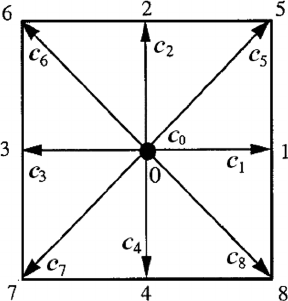
\includegraphics[width=5cm]{img/d2q9}
\end{center}
\begin{center}
  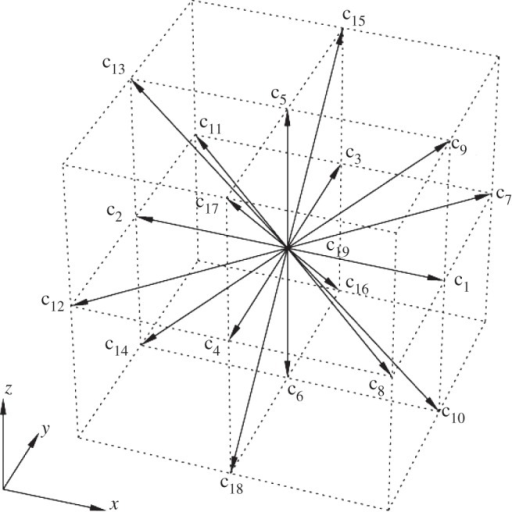
\includegraphics[width=10cm]{img/d3q19}
\end{center}

Diskrete Impulsvektoren für D2Q9:
\[ \vec{p}_i = \xi \cdot \vec{e}_i \]
mit
\begin{align*}
  \vec{e}_0 &= \pmat{0\\0},
            & \vec{e}_1 &= \pmat{-1\\0},
            & \vec{e}_2 &= \pmat{1\\0}, \\
  \vec{e}_3 &= \pmat{0\\-1},
            & \vec{e}_4 &= \pmat{0\\1},
            & \vec{e}_5 &= \pmat{-1\\-1}, \\
  \vec{e}_6 &= \pmat{-1\\1},
            & \vec{e}_7 &= \pmat{1\\-1},
            & \vec{e}_8 &= \pmat{1\\1}.
\end{align*}
Entsprechend gilt die diskretisierte Verteilungsfunktion
\[ f_i(\vec{x}), t) := f( \vec{x}, \vec{p}_i, t) \]
für $t = 0, \ldots, 8$.

Erinnerung: Die Boltzmann-Gleichung (ohne externe Kräfte):
\[ \partial_t f( \vec{x},\vec{p},t) +
  \underbrace{\vec{p} \cdot \nabla f(\vec{x}, \vec{p}, t)}_{\text{Konvektion}}
  = \underbrace{C[f] (\vec{x}, \vec{p}, t)}_{\text{Kollision}}.
\]

Der LBM-Algorithmus behandelt Konvektion und Kollision separat (``splitting'').
Für einen Zeitschritt $t \to t + \Delta t$ berechne
\[ f_i(\vec{x},t) \xrightarrow{\text{Konvektion}}
  f_i^*(\vec{x},t+ \Delta t) \xrightarrow{\text{Kollision}}
  f_i(\vec{x},t+ \Delta t). \]

\subsubsection*{Konvektion}
``stream step''

Idee: Verteilungsfunktion wird entlang diskreter Impulse $\vec{p}_i$ zu den
Nachbarzellen transportiert.
%% Bild
\[ f_i^*(\vec{x},t + \Delta t) = f_i(\vec{x} - \Delta t \vec{p}_i, t) \]
für alle $i = 0, \ldots, 8$.

\subsubsection*{Kollision}
``collision step''

Mehrere Approximationen:
\begin{itemize}
\item Ersetze exakten Kollisionsoperator durch
  Bhatnagar-Gast-Krook-Approximation (BGK): $C[f] \approx C_{\BGK}[f]$ mit
  \[ C_{\BGK}[f] = - \rez{\tau} (f - f_{\MB}), \]
  wobei $\tau$ die Zeitskala der Relaxation ins Gleichgewicht ist, dieser
  Wert wird fest gewählt.
\item Taylor-Entwicklung der Maxwell-Boltzmann-Verteilung $f_{\MB}$
  bezüglich der durchschnittlichen Geschwindigkeit $\vec{u}$.
  \begin{align*}
    f_{\MB}(\vec{p})
    &= \rho \left( \frac{\beta}{2\pi} \right)^{d/2}
      e^{-\beta \rez{2} |\vec{p}|^2} \\
    &= \boxed{
      \rho \left( \frac{\beta}{2\pi} \right)^{d/2}
      e^{-\beta \rez{2} |\vec{p}|^2}
      \left(
      1 + \beta \vec{p} \cdot \vec{u}
      + \rez{2} (\beta \vec{p} \cdot \vec{u})^2
      - \rez{2} \beta |\vec{u}|^2
      \right)
      } + O(u^3) \\
    &=: f^{(\text{eq})}(\vec{p}) + O(u^3),
  \end{align*}
  wobei $d = 2,3$.
\end{itemize}
Die Erhaltungsgrößen bleiben unverändert, das heißt
\[ \int \varphi(\vec{p}) f_{\MB}(\vec{p}) \diffop^3 p
  = \varphi(\vec{p}) f^{(\text{eq})}(\vec{p}) \diffop^3 p \]
für die Kollisionsinvarianten $\varphi(\vec{p}) = 1,
\vec{p}, \rez{2} |\vec{p}|^2$. Der zweidimensionale Fall folgt genauso.

Die Parameter $\rho, \vec{u}, \beta$ in $f_{\MB}$ sollen durch
Erhaltungssätze festgelegt werden. Im konti\-nuierlichen Fall:
\[ \rho = \int f \diffop^3 p, \qquad
  \vec{u} = \rez{\rho} \int \vec{p} f \diffop^3 p, \qquad
  \eps = \ldots \]

\subsubsection*{Adaption auf Diskretisierung $f_i(\vec{x},t)$?} Wir kennen
$f(\vec{x}, \vec{p}, t)$ nur für diskrete Punkte $\vec{p}_i$.

Idee: Konstruiere eine Quadraturformel mit $\vec{p}_i$ als Stützstellen und
$\left( \frac{\beta}{2\pi} \right)^{d/2} e^{-\beta \rez{2} |\vec{p}|^2}$
als Gewichtsfunktion.

Erinnerung: Quadraturformel (in einer Dimension)
\[ \int_a^b h(x) g(x) \diffop x \approx
  \sum_{i=1}^n w_i h(x_i) \]
mit der vorgegebenen Gewichtsfunktion $g(x)$. Die Gewichte $w_i$ und die
Stützstellen $x_i$ werden so gewählt, dass ``$=$'' gilt für Polynome $h$
bis zu einem möglichst hohen Grad.

\subsubsection*{Für Lattice-Boltzmann} Die Stützstellen können nicht frei gewählt
werden, sondern sind genau die diskreten Impulse $\vec{p}_i = \xi \cdot
\vec{e}_i$, $\xi$ ist der einzige freie Parameter.

%% Bild Gewichte

Die Gewichte $w_i$ sollen Isotropie-Bedingungen erfüllen, das heißt sie sollen
invariant unter einer Rotation um \SI{90}{\degree} sein.
\[ w_1 = w_2 = w_3 = w_4, \qquad w_5 = w_6 = w_7 = w_8. \]

Quadraturformel für D2Q9: Es soll gelten
\[ \int h(\vec{p})
  \underbrace{
    \left( \frac{\beta}{2\pi} \right)^{d/2} e^{-\beta \rez{2} |\vec{p}|^2}
  }_{\text{Gewichtsfunktion}}
  \diffop^3 p =
  \sum_{i=0}^8 w_i h(\vec{p}_i)
\]
mit $\vec{p}_i = \xi \vec{e}_i$. $h$ ist ein Polynom in $p_x$ und $p_y$ (zum
Beispiel $h(\vec{p}) = p_x^1 p_y^2 + 1$) bis zum Grad 5.

Lösung: Es muss ein Produkt von modifizierten Gauß-Hermite-Integrationen
bestimmt werden, eine Quadraturformel in jeder Koordinatenrichtung ($p_x, p_y$).
\[ w_0 = \frac{4}{9}, \qquad w_1 = w_2 = w_3 = w_4= \rez{9},
  \qquad w_5 = w_6 = w_7 = w_8 = \rez{36}. \]

Eigentlich: 
$\beta$ (inverse Temperatur) sollte kompatibel mit $f( \vec{x}, \vec{p}, t )$
gewählt werden, sie wird aber hier durch $\xi$ festgelegt. Die Länge einer
Gitterzelle $\xi \Delta t$ kann sich nicht ändern.

Man arbeitet daher mit einer ``isothermalen'' Approximation: Halte die
Temperatur während der Simulation konstant. Dann wird allerdings die
Energieerhaltung verletzt.

\emph{Gebräuchliche Wahl}: Gitterkonstante $\xi \Delta t = 1$, $\Delta t = 1$
und somit auch $\xi = 1$, also $\beta = 3$.

Nun wenden wir die Quadraturformel (in 2D) an:
\begin{align*}
  \int_{\real^2} h(\vec{p}) f(\vec{x}, \vec{p}, t) \diffop^2 p
  &= \int_{\real^2} \underbrace{
    h(\vec{p}) \frac{f(\vec{x}, \vec{p}, t)}
    {\left( \frac{\beta}{2\pi} \right) e^{-\beta \rez{2} |\vec{p}|^2}}
  }_{\tilde{h}(\vec{p})}
  \left( \frac{\beta}{2\pi} \right) e^{-\beta \rez{2} |\vec{p}|^2}
    \diffop^2 p \\
  &\overset{\text{Qu.}}{\approx}
    \sum_{i=0}^8 w_i \tilde{h}(\vec{p}_i) \\
  &= \sum_{i=0}^8 h(\vec{p}_i) \underbrace{ w_i
    \frac{f(\vec{x}, \vec{p}_i, t)}
    {\left( \frac{\beta}{2\pi} \right) e^{-\beta \rez{2} |\vec{p}_i|^2}}
    }_{=: f_i( \vec{x}, t )}.    
\end{align*}
Insbesondere:
\[ \rho = \int_{\real^2} f \diffop^2 p \approx \sum_{i=0}^8 f_i(\vec{x}, t) \]
sowie
\[ \vec{u} = \rez{\rho} \int_{\real^2} \vec{p} f \diffop^2 p \approx
  \rez{\rho} \sum_{i=0}^8 \vec{p}_i f_i(\vec{x}, t) =
  \rez{\rho} \xi \sum_{i=0}^8 \vec{e}_i f_i(\vec{x}, t).
\]
Entsprechend für die Gleichgewichtsverteilung:
\begin{align*}
  f_i^{(\text{eq})}
  &= w_i \frac{f^{(\text{eq})}(\vec{p}_i)}
    {\left( \frac{\beta}{2\pi} \right) e^{-\beta \rez{2} |\vec{p}_i|^2}} \\
  &= w_i \frac{\rho \left( \frac{\beta}{2\pi} \right)
    e^{-\beta \rez{2} |\vec{p}_i|^2} \left( 1 + \beta \vec{p}_i \cdot \vec{u}
    + \rez{2} (\beta \vec{p}_i \cdot \vec{u})^2
    - \rez{2} \beta |\vec{u}|^2 \right) }
    {\left( \frac{\beta}{2\pi} \right) e^{-\beta \rez{2} |\vec{p}_i|^2}} \\
  &= w_i \rho \left( 1 + \beta \vec{p}_i \cdot \vec{u}
    + \rez{2} (\beta \vec{p}_i \cdot \vec{u})^2
    - \rez{2} \beta |\vec{u}|^2 \right),
\end{align*}
wobei $\beta \xi^2 = 3$.

\section*{Zusammenfassung Basis-LBM-Algorithmus}
\begin{itemize}
\item Periodische Randbedingungen
\item Parameter: $\xi$, $\Delta t$, $\tau \in [\rez{2}, \infty)$.
\item Geometrie des Simulationsgebietes: Rechteck (2D) oder Quader (3D)
  bestehend aus gleichförmigen Zellen mit Seitenlänge $\xi \Delta t$.

  Jede Zelle hat diskrete Koordinaten $\vec{x} \in \xi \cdot \Delta t \cdot
  \integer^d$.
\item Anfangsbedingung: Diskretisierte Verteilungsfunktion $f_i(\vec{x}, 0)$ für
  alle Zellen $\vec{x}$, Impulsrichtungen $i = 0, 1, \ldots, 8$ (D2Q9) bzw. $i
  = 0, 1, \ldots, 18$ (D3Q19).
\end{itemize}

Algorithmus: Für $t = 0, \Delta t, 2 \Delta t, \ldots$ \\
Konvektion (``stream step''):
\[ f_i'(\vec{x}, t + \Delta t) = f_i( \vec{x} - \Delta t \vec{p}_i, t) \]
für alle $\vec{x}, i$.

Kollision (``collision step''):
\begin{align*}
  \rho &= \sum_i f_i'(\vec{x}, t + \Delta t), \\
  \vec{u} &= \rez{\rho} \sum_i \vec{p}_i f_i'(\vec{x}, t + \Delta t).
\end{align*}
Bestimme mit $\rho$ und $\vec{u}$ als Parameter die lokale
Gleichgewichtsverteilung:
\[ f_i^{(\text{eq})} = w_i \rho \left( 1 + \beta \vec{p}_i \cdot \vec{u}
    + \rez{2} (\beta \vec{p}_i \cdot \vec{u})^2
    - \rez{2} \beta |\vec{u}|^2 \right), \]
wobei $\beta = \frac{3}{\xi^2}$.
\[ f_i( \vec{x}, t + \Delta t ) = f_i'(\vec{x}, t + \Delta t )
\underbrace{- \rez{\tau} (f_i'(\vec{x},t+\Delta t) - f_i^{(\text{eq})})}_{BGK}\]

\section{Randbedingungen für Hindernisse}
An Wänden und Hindernissen führt man eine Modifikation des Konvektionsschritts
aus.

``no-slip''-Randbedingung (kein Rutschen): Die Impulse in Richtung Wand
werden umgedreht. An rauen Hindernissen (Steinwand) invertiert man
typischerweise die Normal- und Tangentialrichtung.

Bezeichne mit $\tilde{i}$ den Richtungsvektor entgegengesetzt zur Richtung
$\vec{e}_i$, das heißt $\vec{e}_{\tilde{i}} = - \vec{e}_i$. Somit gilt
\[ f_i'(\vec{x}, t + \Delta t) =
  \begin{cases}
    f_{\tilde{i}}(\vec{x}, t), & \text{falls $\vec{e}_{\tilde{i}}$ in Richtung
      Hindernis,} \\
    f_i(\vec{x} - \Delta t \vec{p}_i, t) &\text{sonst.}
  \end{cases}
\]

``free-slip''-Randbedingung (freies Rutschen): Lediglich die Normalenrichtung
wird umgedreht. Das ist typisch für glatte Oberflächen, zum Beispiel Glas.

%% Mehr?

\section*{Berücksichtigung externer Kräfte}
Erinnerung:
\[ \partial_t f + \frac{\vec{p}}{m} \cdot \partial_{\vec{x}} f
  + \vec{F} \cdot \partial_{\vec{p}} f = C[f]. \]
$\vec{F}$ bezeichnet die externe Kraft.

Approximation: Ersetze $\vec{F} \cdot \partial_{\vec{p}} f$ durch $\vec{F} \cdot
\partial_{\vec{p}} f_{\MB} |_{\vec{u}=0}$. Es gilt
\[ \partial_{\vec{p}} |\vec{p}|^2 =
  \pmat{\partial_{p_x} \\ \partial_{p_y} \\ \partial_{p_7}}
  (p_x^2 + p_y^2 + p_z^2)
  = 2 \vec{p} \]
und damit erhalten wir
\[ \begin{aligned}
    \vec{F} \cdot \partial_{\vec{p}} f_{\MB} |_{\vec{u}=0}
    &= \vec{F} \partial_{\vec{p}} \rho \left( \frac{\beta}{2\pi} \right)^{d/2}
    e^{-\beta \rez{2} |\vec{p}|^2} \\
    &= \vec{F} \cdot \left(  \rho \left( \frac{\beta}{2\pi} \right)^{d/2}
      e^{-\beta \rez{2} |\vec{p}|^2} (-\beta \rez{2} 2 \vec{p})
    \right) \\
    &= \underbrace{
      - \rho \beta \left( \frac{\beta}{2\pi} \right)^{d/2}
      e^{-\beta \rez{2} |\vec{p}|^2} (\vec{F} \cdot \vec{p})
      }_{=: \Delta f^{(\text{ext})}(\vec{p})}.
  \end{aligned}
\]
Damit erhalten wir den diskreten und entdimensionalisierten Ausdruck
\[ \Delta f_i^{(\text{ext})} = w_i \frac{\Delta f^{(\text{ext})}(\vec{p}_i)}
  {\left( \frac{\beta}{2\pi} \right)^{d/2} e^{-\beta \rez{2} |\vec{p}|^2}}
  = w_i \rho \beta ( \vec{F} \cdot \vec{p}_i ). \]
Somit: Modifiziere den letzten Schritt im Basis-Algorithmus zu
\[ f_i(\vec{x}, t + \Delta t) = f_i^*(\vec{x},t + \Delta t) - \rez{\tau}( f_i^*
  (\vec{x}, t + \Delta t) -f_i^{(\text{eq})})
  + {\color{red} \Delta f_i^{(\text{ext})}}, \]
wobei $f_i^*$ nach der Konvektion (``stream step'') zu betrachten ist.

\section*{Ausblick: Lattice-Boltzmann für freie Oberflächen}
Typischer Anewndungsfall: Flüssigkeit mit dynamischer Grenzschicht, zum Beispiel
Wasseroberfläche.

$\rightsquigarrow$ Mitverfolgen der Grenzschicht während der Simulation.

%% Bild Oberfläche

Drei Zelltypen:
\begin{itemize}
\item F: Fluidzelle
\item IF: Interface (Grenzschicht)
\item E: Leer (empty)
\end{itemize}

Berechne eine approximative Oberflächennormale $\vec{n}$ basierend auf dem
``Füllstand'' in Zellnachbarschaft.

\section{Image-Inpainting als Navier-Stokes-Gleichung}
\section*{Image-Inpainting}
Kontinuum-Formulierung (Pixelgröße $\to 0$). $\Omega$ sei der gesamte
Bildbereich, der Rekonstruktionsbereich ist $D \subset \Omega$.

Die Bildfunktion $\psi: \Omega \to [0,1]$ liefert Grauwerte (Farbfotos in
mehrere Kanäle auftrennen). Sie ist nur außerhalb von $D$ bekannt.

Idee (Bertalmio und Koautoren 2000, 2001): Virtuelle Zeitevolution (innerhalb
$D$), wobei $\psi(\vec{x},t)$ jetzt zusätzlich von ``virtueller'' Zeit $t$
abhängt.
\[ \partial_t \psi = \vec{N} \cdot \nabla L = \sum_{i=1}^2 N_i \partial_{x_i} L, \]
wobei $\vec{N}$ die Richtung und $L$ die Information, die transportiert werden
soll, bezeichnet. Vergleiche dazu den Konvektionsterm $(\vec{u} \cdot \nabla)
h$.

Intuition: Transport entlang von Konturlinien (``Isophoten''). Diese liegen
senkrecht zum Gradienten $\nabla \psi$. Ein tangentialer Vektor zur Isophote
liegt also auch senkrecht zum Gradient.
\[ \vec{N} = \nabla^\perp \psi, \qquad \nabla^\perp
  = \pmat{-\partial_{x_2} \\ \partial_{x_1}} \]
$\nabla^\perp \psi$ steht senkrecht auf $\nabla \psi$, denn
\[ (\nabla^\perp \psi)(\nabla \psi)
  = \pmat{-\partial_{x_2} \psi \\ \partial_{x_1} \psi}
  \cdot \pmat{\partial_{x_1} \psi \\ \partial_{x_2} \psi} = 0. \]

Glatte Fortsetzung:
\[ L = \Delta \psi, \qquad \Delta = \partial_{x_1}^2 + \partial_{x_2}^2. \]

Somit:
\[ \partial_t \psi = \vec{N} \cdot \nabla L = (\nabla^\perp \psi) \cdot \nabla
  (\Delta \psi). \]
In den Papers von 2000/2001 entwickeln die Autoren einen diskreten Algorithmus,
der für Pixelgröße $\to 0$ auf diese stetige Differentialgleichung führt.

Bemerkung: Eine äquivalente Darstellung ist
\[ \partial_t \psi - \vec{v} \nabla \psi = 0 \]
mit $\vec{v} = \nabla^\perp \Delta \psi$, denn
\begin{align*}
  (\nabla^\perp \psi) \cdot \nabla \Delta \psi
  &= \pmat{-\partial_{x_2} \psi \\ \partial_{x_1} \psi}
  \cdot \pmat{\partial_{x_1} \Delta \psi \\ \partial_{x_2} \Delta\psi} \\
  &= -(\partial_{x_2} \psi)(\partial_{x_1} \Delta \psi)
    +(\partial_{x_1} \psi)(\partial_{x_2} \Delta \psi) \\
  &= \pmat{\partial_{x_2} \Delta \psi \\ -\partial_{x_1} \Delta \psi}
  \cdot \pmat{\partial_{x_1} \psi \\ \partial_{x_2} \psi} \\
  &= - \underbrace{(\nabla^\perp \Delta \psi)}_{\vec{v}} \cdot \nabla \psi.
\end{align*}
Also wird $\psi$ von $\vec{v}$ ``transportiert'' in Richtung der Konturlinien
von $\Delta \psi$.

\section*{Zusammenhang mit Navier-Stokes}
Gegeben: Geschwindigkeitsfold $\vec{u} : \Omega \to \real^2$, divergenzfrei
($\nabla \cdot \vec{u} = 0$). $\vec{u}$ löse die Navier-Stokes-Gleichung
(inkompressibler Fall).

Wirbelstärke:
\[ w = \nabla \times \vec{u} := \partial_{x_1} u_2 - \partial_{x_1} u_1 \]
Das ist die $z$-Komponente der Rotation in drei Dimensionen:
\[ \left[ \pmat{\partial_{x_1} \\ \partial_{x_2} \\ \partial_{x_3}} \times
    \pmat{ u_1 \\ u_2 \\ 0 } \right]_3
  = \partial_{x_1} u_2 - \partial_{x_2} u_1. \]
Definiere $\vec{u}^\perp := \pmat{u_2 \\ -u_1}$, dann gilt:
\[ \nabla \times \vec{u}^\perp = \partial_{x_1}(-u_1) - \partial_{x_2} u_2 =
  - \nabla \cdot \vec{u} = 0. \]
$\vec{u}^\perp$ ist wirbelfrei, kann also als Gradient einer ``Stromfunktion''
$\psi$ dargestellt werden:
\[ \vec{u}^\perp = \nabla \psi, \qquad \vec{u} = \nabla^\perp \psi. \]
Eingesetzt in die Wirbelstärke:
\[ w = \partial_{x_1} u_2 - \partial_{x_2} u_1 = \partial_{x_1} \partial_{x_1}
  \psi - \partial_{x_2} (-\partial_{x_2} \psi) = \Delta \psi. \]

Erinnerung: Navier-Stokes-Gleichung mit konstanter Dichte $\rho(\vec{x},t) = 1$:
\[ \partial_t \vec{u} + (\vec{u} \cdot \nabla) \vec{u} + \nabla P = \mu \Delta
  \vec{u} \]
mit dem Druck $P$ und der Viskosität $\mu$.

Anwenden von $\nabla \times \cdot$ (von links) liefert
\[ \partial_t w + \vec{u} \cdot \nabla w = \mu \Delta w, \]
wobei $\nabla \times (\nabla P) = 0$ aus Aufgabe 11b folgt.

Im stationären Fall ($\partial_t w = 0$) und ohne Viskosität ($\mu = 0$) bleibt
also nur der mittlere Term übrig:
\[ 0 = \vec{u} \cdot \nabla w = (\nabla^\perp \psi) \cdot \nabla \Delta \psi. \]
Das ist genau der Image-Inpainting-Term.

\chapter{Informationssuche im Web: Google's PageRank}
Google: 1998 gegründet von Sergey Brin und Larry Page (Googol: $10^{100}$)

Schwierigkeiten bei der Websuche:
\begin{itemize}
\item Sehr große \emph{Anzahl} von Webseiten (\num{1.3e9} Seiten; Stand Dezember
  2017),
\item nicht sortiert (nach Themenkomplexen),
\item Web-Suche soll für Laien zugänglich sein (``Intention'' der Suche
  erkennen, Tippfehler ausbessern etc.).
\end{itemize}

\section{Grobes Modell einer Suchmaschine}
\begin{enumerate}
\item Suche im ``Index'': Die Suchmaschine generiert aus dem internen
  \emph{Index} (Datenbank) eine unsortierte Trefferliste aller für die
  Suchanfrage relevanten Webseiten (Suchbegriff erscheint auf Webseite).
\item Ranking: Die Trefferliste wird nach Ranking-Faktoren sortiert und
  ausgegeben.
\end{enumerate}

Suchmaschinen ``durchforsten'' das Internet mittels ``Web-Crawlern''
(automatisierte Surfer, ``robots''), die Webseiten herunterladen.

Anschließend parsen sie den Inhalt, zum Beispiel nach der Häufigkeit bestimmter
Wörter oder der Linkstruktur (Verweise auf andere Webseiten). Die Ergebnisse
werden indiziert und in einer Datenbank gespeichert.

\subsection*{Ranking-Faktoren}
\begin{itemize}
\item Kriterien: Relevanz für die Suchanfrage, inhaltliche Qualität.
\item Anfrageabhängige Faktoren: zum Beispiel Häufigkeit des Suchbegriffs auf
  der Seite.
\item Anfrageunabhängige Faktoren: zum Beispiel ``Popularität'' einer Seite,
  ``Klickhäu\-fig\-keit'' oder Verlinkung mit anderen Seiten.

  Vorteil: Diese Faktoren können schon vor der Suchanfrage berechnet werden.
\end{itemize}

\emph{Entscheidende Neuerung in Google's Page-Rank-Algorithmus}: Ausnutzung der
Link\-struk\-tur des Internets.
  
\section{Von der Link-Struktur zum PageRank}
Idee: ``Eine Webseite ist umso wichtiger, je mehr andere wichtige Seiten darauf
verweisen.''

Modellbeispiel:
\begin{center}
  \begin{minipage}{5cm}
    \includegraphics{img/pr_intro}
  \end{minipage}
  \begin{minipage}{9cm}
    \begin{itemize}
    \item $n = 4$ Webseiten $S_i$,
    \item $|S_j|$: Anzahl der ausgehenden Links, $|S_1| = 3$, $|S_2| = 2$, usw.
    \item $B_J$: Menge der auf $S_j$ verweisenden Seiten (``back links''), $B_1
      = \{ S_3, S_4 \}$, $B_2 = \{S_1\}$, usw.
    \end{itemize}
  \end{minipage}
\end{center}
$r_j$: Zu bestimmendes Ranking einer Webseite (``Page Rank'')
\[ r_i = \sum_{S_j \in B_i} \frac{r_j}{|S_j|}, \quad i = 1, \ldots, n. \]

$\Rightarrow$ Indizierung und Speicherung in Datenbank

Selbstreferenziell, Struktur $A \cdot \vec{r} = \vec{r}$.

\subsection*{Matrix-Vektor-Notation}
Hyperlink-Matrix $H \in \realmat{n}{n}$. Einträge:
\[ h_{ij} = \begin{cases}
    \rez{|S_i|}, & S_i \in B_j\footnotemark\\
    0, & \text{sonst.}
  \end{cases}
\]
\footnotetext{$S_i$ besitzt einen Link auf $S_j$.}

Für den PageRank-Vektor gilt
\[ \vec{r}^\top = \vec{r}^\top \cdot H
  \quad \text{bzw.} \quad
  H^\top \cdot \vec{r} = \vec{r},
\]
das heißt $\vec{r}$ ist ein Eigenvektor von $H^\top$ zum Eigenwert 1.

Im Modellbeispiel:
\[ H = \begin{pmatrix}
    0 & \rez{3} & \rez{3} & \rez{3} \\
    0 & 0 & \rez{2} & \rez{3} \\
    1 & 0 & 0 & 0 \\
    \rez{3} & 0 & \rez{3} & 0
  \end{pmatrix}
\]

Linkseigenvektor zum Eigenwert 1:
\[ \vec{r}^\top = (\num{.387}, \num{.129}, \num{.290}, \num{.194}). \]
Alle Einträge sind $\ge 0$, sie können als ``rank'' interpretiert werden. Somit
ist das Ranking der Webseiten:
\[ S_1, S_3, S_4, S_2. \]
Zum Vergleich betrachte das ``naive'' Ranking anhand der Anzahl der eingehenden
Links:
\[ S_3, (S_1, S_4), S_2. \]

Besitzt $H$ stets einen (eindeutigen) Eigenvektor zum Eigenwert 1? Nein!

\subsubsection*{Beispiel für die Nichtexistenz}
\begin{center}
  \begin{minipage}{5cm}
    \includegraphics{img/pr_nonexist}
  \end{minipage}
  \begin{minipage}{9cm}
    $S_3$ hat keine ausgehenden Links.
    \[ H = \begin{pmatrix}
        0 & \rez{2} & \rez{2} \\
        \rez{2} & 0 & \rez{2} \\
        0 & 0 & 0
      \end{pmatrix}
    \]
    Spektrum: $\sigma(H) = \{ \rez{2}, -\rez{2}, 0 \}$. Also ist 1 kein Eigenwert
    von $H$.
  \end{minipage}
\end{center}

\subsubsection*{Beispiel für die Uneindeutigkeit}
\begin{center}
  \begin{minipage}{5cm}
    \includegraphics{img/pr_nonunique}
  \end{minipage}
  \begin{minipage}{9cm}
    Isolierte Inseln
    \[ H = \begin{pmatrix}
        0 & 1 & 0 & 0 \\
        1 & 0 & 0 & 0 \\
        0 & 0 & 0 & 1 \\
        0 & 0 & 1 & 0 
      \end{pmatrix}
    \]
    $\sigma(H) = \{1, 1, -1, -1\}$. Es gibt also mehrere Eigenvektoren zum
    Eigenwert 1.
  \end{minipage}
\end{center}

\section{Diskrete Markov-Ketten}
\begin{itemize}
\item Zustandsraum $Z = \{ 1, 2, \ldots, n \}$. \\
  Zum Beispiel Wetter: $Z = \{ 1, 2 \} =: \{$ ``Sonne'', ``Regen'' $\}$.
\item $X_k$: Zufallsvariable mit Werten in $Z$, für diskrete Zeitpunkte $k = 0, 1,
  \ldots$ \\
  Beispiel $X_5 = 2$: ``Es regnet am fünften Tag''.
\end{itemize}

\subsubsection*{Notation}
\begin{itemize}
\item $\pi_i^k = \pP( X_k = i)$: Wahrscheinlichkeit, dass $X_k$ den Zustand $i$
  annimmt. \\
  Zum Beispiel $\pi_2^5$: Wahrscheinlichkeit, dass es am fünften Tag regnet.
  \[ \pi_i^k \ge 0, \qquad \sum_{i \in Z} \pi^k = 1. \]
\item Der Vektor $\pi^k$ heißt \emph{Zustandsverteilung} zum Zeitpunkt $k$.
\end{itemize}

\subsubsection*{Markov-Eigenschaft}
Wahrscheinlichkeitsverteilung zum Zeitpunkt $k+1$ hängt nur von der
Wahrscheinlichkeitsverteilung am Zeitpunkt $k$ ab:
\[ \pP( X_{k+1} = i_{k+1} | X_k = i_k, X_{k-1} = i_{k-1}, \ldots, X_1 = i_1)
  = \pP( X_{k+1} = i_{k+1} | X_k = i_k ). \]
$p_{ij}$: Übergangswahrscheinlichkeit von Zustand $i$ nach $j$ in einem
Zeitschritt,
\[ p_{ij} = \pP( X_{k+1} = j | X_k = i ) \ge 0. \]
Diese Größe ist unabhängig von $k$ wegen der zeitlichen Translationsinvarianz.
Somit:
\begin{align*}
  \pi_j^{k+1}
  &= \pP (X_{k+1} = j) \\
  &= \sum_{i \in Z} \underbrace{\pP(X_{k+1} = j | X_k = i)}_{=p_{ij}} \cdot
    \underbrace{\pP(X_k = i)}_{= \pi_i^k} \\
  &= \sum_{i \in Z} \pi_i^k p_{ij}.
\end{align*}
Matrix-Vektor-Notation:
\[ \pi^{k-1} = P^\top \pi^k, \qquad P := (p_{ij}). \]
$P$ ist eine \emph{Rekursionsmatrix}, es gilt
\[ \pi^{k+1} = P^\top \pi^k = P^\top P^\top \pi^{k-1} = \cdots = (P^\top)^{k+1}
  \pi^0. \]
Außerdem ist $P$ eine \emph{stochastische Matrix}:
\[ p_{ij} \ge 0, \qquad \sum_{j \in Z} p_{ij} = 1 \text{ für alle } i. \]
Begründung:
\begin{align*}
  \sum_{j \in Z} p_{ij}
  &= \sum_{j \in Z} \pP( X_{k+1} = j | X_k = i ) \\
  &= \pP( X_{k+1} \in Z | X_k = i ) = 1.
\end{align*}
Eine Zustandsverteilung $\pi$ heißt \emph{stationär} bzw.
\emph{Gleichgewichtsverteilung}, falls
\[ P^\top \pi = \pi, \]
das heißt $\pi$ ist Eigenvektor von $P^\top$ zum Eigenwert 1 und ein Fixpunkt
der Iterationsvorschrift
\[ \pi^{k+1} = P^\top \pi^k. \]

\subsubsection*{Bedingungen an $P$, sodass
  $\lim_{n \to \infty} (P^\top)^{k+1} \pi^0$ existiert?}
$P$ ist eine stochastische Matrix, also gilt mit $e = (1, 1, \ldots, 1)^\top$
\[ P \cdot e = e, \]
das heißt $P$ besitzt einen Eigenvektor zum Eigenwert 1. Wegen
\[ \sigma( P^\top ) = \sigma( P ) \]
mit $\sigma =$ Menge der Eigenwerte\footnote{%
  Das kann man zum Beispiel mit dem charakteristischen Polynom beweisen.
} ist 1 auch ein Eigenwert von $P^\top$.

\textbf{Spektralradius:}
\[ \rho( P ) := \max\{ | \lambda | : \lambda \in \sigma(P) \}. \]
Es gilt
\[ 1 \le \rho(P) \le \| P \|_{\infty}, \]
wobei
\[ \| P \|_{\infty} = \max_{i \in Z} \sum_{j \in Z} p_{ij} = 1 \]
nach Definition. Also gilt
\[ \rho( P ) = \rho( P^\top ) = 1. \]
Somit ist 1 der dominante Eigenwert, aber es ist a priori nicht klar, ob ein
zugehöriger Eigenvektor mit Einträgen $\ge 0$ existiert.

Eine hinreichende Bedingung ist durch den folgenden Satz gegeben:
\begin{thm}[Perron-Frobenius]
  Sei $A \in \realmat{n}{n}$ eine Matrix mit strikt positiven
  Einträgen\footnotemark, dann gilt:
  \begin{enumerate}[a)]
  \item $A$ hat einen strikt dominanten positiven Eigenwert $\lambda_1 > 0$, den
    sogenannten \emph{Perron-Eigenwert}.
  \item Es gibt einen Eigenvektor\footnotemark $v_1$ zu $\lambda_1$ 
    mit strikt positiven Einträgen.
  \item Der Perron-Eigenwert ist algebraisch einfach\footnotemark.
  \item Außer $v_1$ gibt es keine weiteren Eigenvektoren\footnotemark von $A$
    mit ausschließlich nicht-negativen Einträgen.
  \end{enumerate}
\end{thm}
\addtocounter{footnote}{-3}
\footnotetext{Das heißt $a_{ij} > 0$ für alle $i$, $j$.}
\addtocounter{footnote}{1}
\footnotetext{$A v_1 = \lambda_1 v_1$.}
\addtocounter{footnote}{1}
\footnotetext{Also ist der Eigenraum eindimensional.}
\addtocounter{footnote}{1}
\footnotetext{Bis auf skalare Vielfache von $v_1$.}

Damit folgt: Falls die stochastische Matrix $P$ zusätzlich $p_{ij} > 0$ für alle
$i$, $j$ erfüllt, dann hat sie den Perron-Eigenwert $\lambda_1 = 1$ und es
existiert eine eindeutige stationäre Verteilung $\pi$.

Außerdem konvergiert die Iterationsvorschrift
\[ \pi^{k+1} = P^\top \pi^k \]
für beliebiges $\pi^0$ gegen $\pi$:
\[ \pi  = \lim_{k \to \infty} \pi^k. \]

Begründung:
\begin{thm}
  Es sei $\lambda_1$ ein algebraisch einfacher, strikt dominanter Eigenwert
  einer Matrix $A \in \complex^{n \times n}$ mit zugehörigem Eigenvektor $v_1$
  und Linkseigenvektor\footnotemark $w_1$ mit
  \[ w_1^\top v_1 = 1. \]
  Dann gilt für den Iterationsprozess
  \[ z^{k+1} = A z^k, \qquad k = 0, 1, 2, \ldots \]
  dass
  \[ \lim_{k \to \infty} \frac{z^k}{\lambda_1^k} = (w_1^\top \cdot z^0) v_1. \]
\end{thm}
\footnotetext{Also $w_1^top A = \lambda_1 w^\top$ bzw.
  $A^\top w_1 = \lambda_1 w_1$.}

\begin{proof}
  Der Beweis wird für diagonalisierbares $A$ geführt. Der Satz gilt auch
  anderenfalls, dann muss man die Jordan'sche Normalform verwenden.

  Seien $v_1, \ldots, v_n$ eine Basis aus Eigenvektoren mit zugehörigen (nicht
  notwendigerweise verschiedenen) Eigenwerten $\lambda_1, \ldots, \lambda_n$.

  Schreibe den Anfangszustand $z^0$ als Linearkombination
  \[ z^0 = \alpha_1 v_1 + \ldots + \alpha_n v_n, \]
  dann gilt
  \begin{align*}
    z^k &= A z^{k-1} = A^2 z^{k-2} = \cdots = A^k z^0 \\
        &= \sum_{i=1}^n \alpha_i \underbrace{A^k v_i}_{\lambda_i^k v_i},
  \end{align*}
  somit
  \[ \frac{z^k}{\lambda_1^k} = \sum_{i=1}^n \alpha_i
    \frac{\lambda_i^k}{\lambda_1^k} v_i
    \xrightarrow{k \to \infty}
    \alpha_1 v_1, \]
  weil
  \[ \frac{\lambda_i^k}{\lambda_1^k} \xrightarrow{k \to \infty}
    \begin{cases}
      1, & i = 1, \\
      0, & i > 1, 
    \end{cases}
  \]
  aufgrund der strikten Dominanz von $\lambda_1$.

  Außerdem
  \begin{align*}
    w_1^\top A v_i &= w_1^\top (\lambda_i v_i) = \lambda_i w_i^\top v_i, \\
    w_1^\top A v_i &= (w_1^\top A) v_i = (\lambda_1 w_1^\top) v_i 
  \end{align*}
  und damit
  \[ (\lambda_i - \lambda_1) w_1^\top v_i = 0. \]
  Wegen $\lambda_i \ne \lambda_1$ für alle $i > 1$ folgt also
  \[ w_1^\top v_i = 0 \quad \text{für alle } i > 1 \]
  und damit
  \[ w_1^\top z^0 = \alpha_1 \underbrace{w_1^\top v_1}_{= 1} = \alpha_1.
    \qedhere \]
\end{proof}

Anwendung des Satzes auf die stochastische Matrix $P^\top$ mit $p_{ij} > 0$ für
alle $i$, $j$:
\[ \lambda_1 = 1, \quad v_1 = \pi\footnotemark, \quad
  w_1 = e = \pmat{1 \\ \vdots \\ 1}, \]
denn $e^\top \pi = \sum_{i \in Z} \pi = 1$ nach Definition. Somit gilt für
beliebige Anfangsverteilungen $\pi^0$:
\[ \lim_{k \to \infty} \pi^k = \underbrace{e^\top \pi^0}_{=1} \pi. \]

\section{Stochastische Interpretation (Zufallssurfer)}
\textbf{Idee:} PageRank ist proportional zur durchschnittlichen Verweildauer
eines Zufallssurfers auf einer Webseite.
\begin{itemize}
\item Zustandsraum $Z$: Menge aller Webseiten,
\item Zufallsvariable $X_k$: $k$-te besuchte Webseite des Zufallssurfers.
\end{itemize}

\textbf{Annahmen:} Der Zufallssurfer ist gedächtnislos, das heißt sein Verhalten
hängt nur von der aktuell besuchten Webseite ab (entspricht der
Markov-Eigenschaft). Der Zufallssurfer bewegt sich zur nächsten Seite, indem er
\begin{enumerate}[a)]
\item zufällig (gleichverteilt) einen der Links auf der aktuellen Seite
  verwendet (falls Links vorhanden sind)
\item zufällig (gleichverteilt) auf eine beliebige Webseite springt (falls
  keine Links auf der aktuellen Seite vorhanden sind)
\end{enumerate}

Damit ergibt sich die Übergangswahrscheinlichkeit
\[ q_{ij} = \pP( X_{k+1} = S_j | X_k = S_j ) =
  \begin{cases}
    \rez{|S_j|}, & S_i \text{ besitzt einen Link auf } S_j, \\
    \rez{n}, & S_i \text{ besitzt keine Links,} \\
    0, & \text{sonst.}
  \end{cases}
\]
Matrixschreibweise:
\[ Q = H + \rez{n} \cdot d e^\top \]
mit
\[ e = \pmat{1 \\ \vdots \\ 1}, \qquad d
  \in \real^n, \quad
  d_i = \begin{cases}
    1, & S_i \text{ besitzt keine Links,} \\
    0, & \text{sonst.}
  \end{cases}
\]
$Q = (q_{ij})$ ist sehr ähnlich zur Hyperlink-Matrix $H$ (außer, wenn keine
Links vorhanden sind). Der Term $\rez{n} d e^\top$ ersetzt Nullzeilen in $H$
durch $(\rez{n}, \rez{n}, \ldots, \rez{n})$.

$Q$ ist eine stochastische Matrix, es gilt $q_{ij} \ge 0$ und für alle $i$ ist
$\sum_{j \in Z} q_{ij} = 1$.

\textbf{Wunsch:} Die Vektoriteration
\[ \pi^{k+1} = Q^\top \pi^k \]
soll gegen die stationäre Grenzverteilung $\pi$ konvergieren, also
\[ \pi = \lim_{k \to \infty} \pi^k, \qquad Q^\top \pi = \pi \]
mit $\pi_i \ge 0$, $\sum_{i=1}^n \pi_i = 1$. Das impliziert
\[ \pi_i = \lim_{l \to \infty} \rez{l} \sum_{k=0}^{l-1} \pi_i^k, \]
wobei $\rez{l} \sum_{k=0}^{l-1} \pi_i^k$ die durchschnittliche
Aufenthaltswahrscheinlichkeit nach $l$ Schritten ist.

\emph{Aber:} $\lim \pi^k$ existiert im Allgemeinen gar nicht. Siehe zum Beispiel
Übungsaufgabe 16(c).

\emph{Erinnerung:} Voraussetzung im Satz von Perron-Frobenius war, dass alle
Matrixeinträge strikt positiv sind.

\textbf{Idee:} (Brin, Page) Modifiziere den Zufallssurfer, sodass er mit einer
kleinen Wahrscheinlichkeit auf eine beliebige Webseite springen kann
(``Teleportation'').

Damit bewegt sich der ``Google''-Zufallssurfer zur nächsten Webseite, indem er
mit Wahrscheinlichkeit $\alpha$ ($0 < \alpha < 1$)
\begin{enumerate}[a)]
\item zufällig (gleichverteilt) einen der Links auf der aktuellen Seite
  verwendet (falls Links vorhanden sind)
\item zufällig (gleichverteilt) auf eine beliebige Webseite springt (falls
  keine Links auf der aktuellen Seite vorhanden sind)
\end{enumerate}
und mit Wahrscheinlichkeit $1 - \alpha$ zufällig mit dem
Wahrscheinlichkeitsverteilungsvektor
\[ v, \quad v_i > 0, \quad \sum_{i=1}^n v_i = 1 \]
auf eine beliebige Webseite springt.

1998 wurde $v = \rez{n} e$ mit $n$ der Gesamtzahl aller Webseiten verwendet.
Heute ist die Struktur von $v$ ein Firmengeheimnis.

\subsubsection*{Entsprechende Google-Übergangsmatrix}
\[ G = \alpha Q + (1-\alpha) e v^\top \]
Schreibweise:
\[ ev^\top = \pmat{1 \\ \vdots \\ 1} (v_1, \ldots, v_n) =
  \begin{pmatrix}
    v_1 & \cdots & v_n \\
    \vdots & & \vdots \\
    v_1 & \cdots & v_n
  \end{pmatrix}.
\]
$G$ ist wiederum eine stochastische Übergangsmatrix. Für die Einträge gilt
$g_{ij} \ge 0$ (sogar $> 0$, da $v_i > 0$ für alle $i$) und
\[ \sum_{j} g_{ij} = \alpha \sum_{j} g_{ij} + (1-\alpha) \sum_{j} v_j
  = \alpha + (1-\alpha) = 1. \]
Somit ist der Satz von Perron-Frobenius anwendbar. Der Perron-Eigenwert ist
$\lambda_1 = 1$ und der entsprechende Eigenvektor $\pi$ ist die eindeutige
Lösung von
\[ G^\top \pi = \pi \quad \text{mit } \sum_{i} \pi_i = 1 \]
und erfüllt $\pi_i > 0$ für alle $i$.

\textbf{Interpretation:} $\pi_i$ ist die durchschnittliche Aufenthaltsdauer des
Google-Zufallssurfers auf der Webseite $S_i$ und wird als PageRank verwendet.

Außerdem: (siehe oben) Die Vektoriteration
\[ \pi^{k+1} = G^\top \pi^k \]
mit beliebiger Anfangsverteilung $\pi^0$  konvergiert gegen $\pi$:
\[ \pi = \lim_{k \to \infty} \pi^k. \]

\subsubsection*{Beispiel}
\begin{center}
  \begin{minipage}{8cm}
    \includegraphics{img/pr_exmp}
  \end{minipage}
  \begin{minipage}{5cm}
    Hyperlink-Matrix:
    \[ H = \begin{pmatrix}
        0 & 0 & 1 & 0 & 0 & 0 \\
        1 & 0 & 0 & 0 & 0 & 0 \\
        0 & 1 & 0 & 0 & 0 & 0 \\
        0 & 0 & 0 & 0 & \rez{2} & \rez{2} \\[.3em]
        0 & 0 & \rez{3} & \rez{3} & 0 & \rez{3} \\[.3em]
        0 & 0 & 0 & 1 & 0 & 0
      \end{pmatrix}
    \]
  \end{minipage}
\end{center}
Es gibt keine ``hängenden Knoten'', jede Seite besitzt mindestens einen Link.
Somit gilt
\[ Q = H. \]

Google-Matrix für $\alpha = \frac{4}{5}$ und $v = \rez{6} e$:
\begingroup
\renewcommand*{\arraystretch}{1.5}
\begin{align*}
  G &= \frac{4}{5} Q + \rez{5} \cdot \rez{6} e e^\top \\
    &= \begin{pmatrix}
      \rez{30} & \rez{30} & \frac{5}{6} & \rez{30} & \rez{30} & \rez{30} \\
      \frac{5}{6} & \rez{30} & \rez{30} & \rez{30} & \rez{30} & \rez{30} \\
      \rez{30} & \frac{5}{6} & \rez{30} & \rez{30} & \rez{30} & \rez{30} \\
      \rez{30} & \rez{30} & \rez{30} & \rez{30} & \frac{13}{30} & \frac{13}{30} \\
      \rez{30} & \rez{30} & \frac{3}{10} & \frac{3}{10} & \rez{30} & \rez{30} \\
      \rez{30} & \rez{30} & \rez{30} & \frac{5}{6} & \rez{30} & \rez{30}
    \end{pmatrix}
\end{align*}
\endgroup
PageRank-Vektor $G^\top \pi = \pi$:
\[ \pi = (\num{.2001}, \num{.2085}, \num{.2189},
  \num{.1557}, \num{.0956}, \num{.1211} )^\top. \]
Damit ist das Ranking der Webseiten:
\[ 3, 2, 1, 4, 6, 5. \]

Zum Vergleich: Für $\alpha = 1$, also $G = H$, erhalten wir
\[ \pi = \left( \rez{3}, \rez{3}, \rez{3}, 0, 0, 0 \right)^\top. \]
Also hätten die Seiten 4, 5 und 6 den PageRank 0.

\section{Berechnung des PageRank-Vektors}
Erste Idee: Löse
\[ G^\top \pi = \pi, \qquad
  e^\top \pi = 1 \]
direkt. Also
\begin{align*}
  (\alpha Q + (1-\alpha) ev^\top)^\top \pi &= \pi \\
  \alpha Q^\top \pi + (1-\alpha) v \underbrace{e^\top \pi}_{=1} &= \pi \\
  (I - \alpha Q^\top) \pi &= (1-\alpha) v.
\end{align*}
Das ist ein lineares Gleichungssystem für $\pi$. Man benötigt für eine dünn
besetzte Matrix $Q$ eine Rechenzeit von $O(n^2)$, also ist das Verfahren nicht
durchführbar für $n \approx 10^9$ Webseiten.

Stattdessen: Führe die Vektoriteration
\[ \pi^{k+1} = G^\top \pi^k, \qquad k = 0, 1, 2, \ldots \]
mit $\pi^0 = \rez{n} e$ aus.

Um das explizite Aufstellen der Matrix $G$ zu vermeiden, können wir $G^\top
\pi^k$ auswerten:
\begin{align*}
  G^\top \pi^k
  &= (\alpha Q^\top + (1-\alpha)ve^\top) \pi^k \\
  &= \alpha Q^\top \pi^k + (1-\alpha) ve^\top \pi^k \\
  &= \alpha H^\top \pi^k + \alpha \rez{n} e(d^\top \pi^k) + (1-\alpha) v,
\end{align*}
wobei $d^\top \pi^k$ ein Skalarprodukt ist.

Somit muss nur das Matrix-Vektorprodukt $H^\top \pi^k$ mit der dünn besetzten
Hyperlink-Matrix $H$ berechnet werden, die Kosten sind $O(n)$.

In der Praxis (laut Brin, Page) benötigt man 50 bis 100 Iterationen. Die
Berechnung von $\pi$ dauert einige Tage.

\subsubsection*{Konvergenzgeschwindigkeit der Vektoriteration}
Die Konvergenz hängt vom Verhältnis der betragsmäßig größten Eigenwerte
$\lambda_1$ und $\lambda_2$ ab:
\[ \| \pi^k - \pi \|_1 \le c \left( \frac{|\lambda_2|}{|\lambda_1|} \right)^k \]
mit einer von $k$ unabhängigen Konstante $c$.

Für die Google-Matrix gilt $\lambda_1 = 1$ und laut Perron-Frobenius ist
$\lambda_1$ strikt dominant, das heißt $|\lambda_2| < |\lambda_1|$.

Frage: Um wie viel ``kleiner'' ist $|\lambda_2|$?

\emph{Behauptung:} Alle anderen Eigenwerte $\lambda \ne 1$ erfüllen
\[ |\lambda| \le \alpha. \]

\begin{proof}
  Sei $u$ ein Eigenvektor von $G^\top$ zum Eigenwert $\lambda$, also
  \[ G^\top u = \lambda u. \]
  Dann gilt
  \[ e^\top( G^\top u ) = \lambda e^\top u \]
  sowie
  \[ (e^\top G^\top)u = (Ge)^\top u = e^\top u. \]
  Also bilden wir die Differenz
  \[ 0 = (\lambda - 1) e^\top u \qRq e^\top 0, \]
  weil $\lambda \ne 1$. Damit folgt
  \[ G^\top u = \alpha Q^\top u + (1-\alpha) v \underbrace{e^\top u}_{=0}
    = \alpha Q^\top u \]
  und es gilt
  \[ \lambda u = \alpha Q^\top u
    \quad \text{bzw.} \quad
    Q^\top u = \frac{\lambda}{\alpha} u.
  \]
  Also ist $\frac{\lambda}{\alpha}$ ein Eigenwert von $Q^\top$ und es folgt
  \[ \left| \frac{\lambda}{\alpha} \right| \le \rho(Q) = 1. \qedhere \]
\end{proof}
Begründung für den Spektralradius $\rho(Q) = 1$: $Q$ ist eine stochastische
Matrix, das heißt sie besitzt den Eigenwert 1 wegen $Qe = e$ und damit
\[ 1 \le \rho(Q) \le \|Q\|_\infty = \max_i \sum_j |q_{ij}| = 1. \]

\subsubsection*{Herleitung der Konstante $c$}
\[ \| \pi^k - \pi \|_1 \le
  \alpha^k \| \pi^0 - \pi \|_1 \le
  \alpha^k (\|\pi^0\|_1 + \|\pi\|_1) = 
  2 \alpha^k, \]
also ist $c = 2$.

Die Konvergenzgeschwindigkeit ist exponentiell in $k$. Für eine Genauigkeit von
$d$ Dezimalstellen muss
\[ 2 \alpha^k \overset{!}{\le} 10^{-d} \]
gelten. Bilden des Logarithmus und Auflösen nach $k$ liefert
\begin{align*}
  \log 2 + k \cdot \log \alpha
  &\le - d \cdot \log 10 \\
  k
  &\ge - \frac{d \cdot \log 10 + \log 2}{\log \alpha}
\end{align*}
wegen $\log \alpha < 0$.

\subsubsection*{Beispiel}
$d = 5$ Stellen:
\begin{center}
  \begin{tabular}{r|cccccc}
    $\alpha$ & \num{.5} & \num{.75} & \num{.8} & \num{.85} & \num{.9} & \num{.99} \\
    $k$ & 18 & 43 & 55 & 76 & 116 & 1215
  \end{tabular}
\end{center}
Die Anzahl der benötigten Iterationen wächst sehr schnell für $\alpha \to 1$.
Eine kleine Teleportationswahrscheinlichkeit $(1-\alpha)$ repräsentiert aber die
tatsächliche Link-Struktur besser.

Google 1998: $\alpha = \num{.85}$, ca. 50 Iterationen.
\[ 2 \cdot \num{.85}^{50} = \num{.00059}\ldots, \]
also nur etwa drei Stellen Genauigkeit.

Aber: Nur die Rangfolge ist interessant, neben dem PageRank werden noch weitere
inhaltsbasierte Kriterien zum Sortieren der Suchergebnisse verwendet. Es muss
also keine sehr hohe Genauigkeit bei der Berechnung des PageRank-Vektors $\pi$
erreicht werden.

\section{Sensitivitätsanalyse des PageRank-Vektors}
\subsubsection*{Sensitivität bezüglich $\alpha$}
Betrachte die Google-Matrix $G$ und den entsprechenden PageRank-Vektor als
Funktion von $\alpha$. Man kann zeigen: $\pi(\alpha)$ ist eine differenzierbare
Funktion und
\[ \left\| \diff{\pi(\alpha)}{\alpha} \right\|_1 \le \frac{2}{1-\alpha}. \]
Somit reagiert $\pi(\alpha)$ nicht allzu sensitiv auf Änderungen von $\alpha$,
so lange $\alpha$ nicht zu nahe bei 1 liegt.

Andererseits ist die Abschätzung für $\alpha \to 1$ nicht aussagekräftig, da
dann $\frac{2}{1-\alpha} \to \infty$. Es stellt sich aber heraus, dass
$\pi(\alpha)$ in der Tat sehr empfindlich bezüglich Änderungen von $\alpha$ ist.

\subsubsection*{Sensitivität bezüglich $H$}
Hier betrachten wir der Einfachheit halber nur das Hinzufügen oder Entfernen von
Links zwischen bestehenden Webseiten\footnote{Das heißt, die Einträge von $H$
  ändern sich.}, nicht aber das Hinzufügen oder Entfernen von Webseiten an sich.

Fasse den PageRank-Vekor als Funktion von $H$ auf, $\pi(H)$. Ziel ist die
Ableitung von $\pi$ bezüglich eines Matrix-Eintrags $h_{ij}$:
\[ \diff{\pi}{h_{ij}}. \]
Ausgangspunkt:
\[ G^\top \pi = \pi, \qquad e^\top \pi = \sum_{i=1}^n \pi_i = 1. \]
Einsetzen von $G = \alpha Q + (1-\alpha) ev^\top$:
\begin{align*}
  (I - \alpha Q^\top) \pi
  &= (1-\alpha) v \\
  \pi
  &= (1-\alpha) (I - \alpha Q^\top)^{-1} v.
\end{align*}

\subsubsection*{Allgemein: Ableitung einer inversen Matrix}
Sei $A(t) \in \realmat{n}{n}$ eine stetig differenzierbare, matrixwertige
Funktion von $t$ und sei $A(t)$ invertierbar für alle $t \in \real$. Ziel ist,
$\diff{}{t} A(t)^{-1}$ zu ermitteln.
\begin{align*}
  0
  &= \diff{}{t} I = \diff{}{t} (A(t) A(t)^{-1} ) \\
  &= \left( \diff{}{t} A(t) \right) A(t)^{-1} + A(t) \diff{}{t} A(t)^{-1}
\end{align*}
nach der Produktregel. Also
\[ \diff{}{t} A(t)^{-1} = - A(t)^{-1} \left( \diff{}{t} A(t) \right)
  A(t)^{-1}. \]

\subsubsection*{Ableitung von $\pi(H)$}
Hier ist $t = h_{ij}$, es gilt
\[ A(h_{ij}) = I - \alpha Q^\top
  = I - \alpha \left( H^\top + \rez{n} ed^\top \right). \]
Also ist
\[ \diff{}{h_{ij}} A(h_{ij}) = - \alpha
  \begin{pmatrix}
    0 & 0 & \cdots \\
    0 & \cdots \\
    & \cdots & 1 & 0 \\
    & & \cdots & 0 \\
  \end{pmatrix}
  = - \alpha \hat{e}_j \hat{e}_i^\top
\]
mit
\[ \hat{e}_i = (\underbrace{0, \cdots, 0}_{i-1 \text{ mal}},
  1, 0, \cdots, 0)^\top. \]

Damit folgt
\begin{align*}
  \diff{\pi}{h_{ij}}
  &= -(1-\alpha) A(h_{ij})^{-1} \left( \diff{}{h_{ij}} A(h_{ij}) \right)
    A(h_{ij})^{-1} v \\
  &= (1-\alpha) (I - \alpha Q^\top)^{-1} (\alpha \hat{e}_j \hat{e}_i^\top)
    (I - \alpha Q^\top)^{-1} v \\
  \intertext{Beachte $(1-\alpha)(I-\alpha Q^\top) v = \pi$:}
  &= \alpha (I - \alpha Q^\top)^{-1} \hat{e}_j
    \underbrace{\hat{e}_i^\top \pi}_{= \pi_i} \\
  &= \alpha \pi_i (I - \alpha Q^\top)^{-1} \hat{e}_j
\end{align*}

Die Matrix-Vektor-Multiplikation $(I - \alpha Q^\top)^{-1} \hat{e}_j$ ergibt die
$j$-te Spalte von $(I-\alpha Q^\top)^{-1}$.

Erinnerung:
\[ h_{ij} = \begin{cases}
    \rez{|S_i|}, & S_i \text{ besitzt Link auf } S_i, \\
    0, & \text{sonst.}
  \end{cases}
\]

\subsubsection*{Interpretation}
$\pi$ ist umso sensitiver bezüglich Einfügen oder Entfernen eines Links von
$S_i$ nach $S_j$, je größer $\pi_i$ ist.

Wegen $\rho(Q^\top) = 1$ ist $I - \alpha Q^\top$ fast singulär für $\alpha \to
1$, die Einträge von $(I - \alpha Q^\top)^{-1}$ divergieren für $\alpha \to 1$.

Somit ist $\pi$ sehr sensitiv bezüglich Link-Änderung für $\alpha \to 1$ (auch,
falls $\pi_i$ klein ist).

\section{Ausblick: Verfeinerung und Verbesserung der Google-Suche}
Google 20 Jahre nach Gründung

\subsubsection*{1. Analyse der Suchanfrage}
Sprachmodell zum ``Verstehen'' der Suchanfrage:
\[ \text{``How to } \underbrace{\text{change}}_{= \text{ replace}} \text{ a
    light bulb''} \]
und Kategorisierung der Suchanfrage: Spezifische Anfrage?

\subsubsection*{2. Abgleich des Suchbegriffs: Suche im ``Index''}
Bei Webseiten, die den Suchbegriff enthalten, wird zusätzlich berücksichtigt, wo
auf der Seite der Begriff vorkommt (im Titel, Haupttext?).

Das wirkt sich auf die Relevanz für die Suchanfrage aus. Zum Beispiel Begriff
``Hunde'' sollte Seiten mit Bildern von Hunden, verschiedenen Hunderassen
liefern, nicht nur das Wort ``Hunde'' auf der Webseite.

\subsubsection*{3. Ranking}
Neben dem PageRank gibt es mittlerweile viele andere Faktoren:
\begin{itemize}
\item Aktualität des Inhalts einer Webseite
\item Nutzerfreundlichkeit der Seite
\item Präferenz anderer Benutzer (welche aufgeführten Seiten werden von anderen
  Nutzern bevorzugt?)
\item Erkennung von Spam-Seiten (künstliche PageRank-Optimierung)
\end{itemize}

\subsubsection*{4. Kontextbezug}
``Personalisierte Suchergebnisse'' basierend auf Standort, Land
\[ \text{``football''} \quad
  \begin{cases}
    \text{American Football} \\
    \text{Fußball}
  \end{cases}
\]
Frühere Suchanfragen (``Barcelona vs. Arsenal'' $\rightsquigarrow$
fußballinteressiert) beeinflussen nachfolgende Suchen (``Barcelona'' liefert
Fußballverein statt der Stadt)

\subsubsection*{5. Zusammenstellung der Ergebnisse}
Ausgewogenheit zwischen eng definierten oder breit gefassten Themen

\chapter{Diskretisierung partieller Differentialgleichungen}
Partielle Differentialgleichungen (PDE) treten in fast allen quantitativen
Naturwissenschaften auf.

\section{Exemplarische Beispiele partieller Differentialgleichungen}
\subsubsection*{Beispiel 1: Stationäres elliptisches Problem}
$u(x) \in \real^d$, $s \in \Omega \subseteq \real^m$ Ortsvariable (oft $m = 2,
3$).

An $\partial \Omega$ werden Daten vorgegeben, etwa
\[ u |_{\partial \Omega} = 0, \qquad \pdiff{u}{n} = 0, \qquad \ldots \]

Anwendung: Form einer Seifenblase

Gegeben sei die Höhe des Drahtes als Funktion $\varphi: \partial \Omega \to
\real$.

Gesucht ist die Höhe $u: \Omega \to \real$ der Seifenblase.

Physikalisches Prinzip der Seifenblasenhaut: Minimierung der Oberfläche
\[ J := \int_\Omega \sqrt{1 + (\partial_{x_1} u)^2 + (\partial_{x_2} u)^2}
  \diffop^2 x \to \min. \]

%% Hopp

Plateau'sches Problem:
\[ \left\{ \quad \begin{aligned}
      &J \to \min \\
      &\text{Randbedingung } u|_{\partial \Omega} = \varphi
    \end{aligned}
  \right.
\]

Bei kleinen Gradienten:
\[ \sqrt{ 1 + (\partial_{x_1} u)^2 + (\partial_{x_2} u)^2}
  \approx
  1 + \rez{2} ((\partial_{x_1} u)^2 + (\partial_{x_2} u)^2). \]
Damit lässt sich das Problem vereinfachen:
\[ \left\{ \quad \begin{aligned}
      &J := \rez{2} \int_\Omega (\partial_{x_1} u)^2 + (\partial_{x_2} u)^2
      \diffop x \to \min \\
      &u|_{\partial \Omega} = \varphi
    \end{aligned}
  \right.
\]
Mit der Euler-Lagrange-Gleichung der Variationsrechnung erhält man
\[ \left\{ \quad \begin{aligned}
      &\partial_{x_1} u)^2 + (\partial_{x_2} u)^2 = 0 \\
      &u|_{\partial \Omega} = \varphi
    \end{aligned}
  \right.
\]
Schreibweise: $\Delta u = 0$.

\subsubsection*{Beispiel 2: Hyperbolische Kontinuitätsgleichung}
\begin{itemize}
\item $\rho(x,t) \in \real$: Dichte
\item $u(x,t) \in \real^2$: Geschwindigkeitsfeld
\end{itemize}

Massenerhaltung:
\begin{align*}
  \pdiff{}{t} \int_V \rho \diffop^3 x
  &= - \int_{\partial V} \rho( u \cdot n ) \diffop^2 S, \\
  \begin{aligned}
    &\text{Zeitliche Änderung} \\
    &\text{der Masse in $V$}
  \end{aligned}
  &= \begin{aligned}
    &\text{Flüssigkeit, die in das Volumen} \\
    &\text{hinein bzw. herausströmt}
  \end{aligned}
\end{align*}

Gauß:
\[ \int_{\partial V} \rho(u \cdot n) \diffop^2 S
  = \int_V \nabla \cdot (\rho u) \diffop^3 x. \]
Weil $V$ beliebig ist:
\[ \pdiff{}{t} \rho + \nabla \cdot (\rho u) = 0. \]
Das ist die Kontinuitätsgleichung für die Dichte.

``hyperbolisch'': Orts- und Zeitableitung haben dieselbe Ordnung, hier 1.

\subsubsection*{Beispiel 3: Parabolische Wärmeleitungsgleichung}
$u(x,t) \in \real^d$, $x \in \real^d$, $d = 1,2,3$.
\[ \partial_t u = k \Delta u \]
mit dem Laplace-Operator $\Delta u = \sum_{i=1}^d \partial_{x_i}^2 u$.

Cauchy-Problem (Anfangs- und/oder Randbedingungen vorgegeben):
\[ u(x, t = 0) = u_0(x) \]

Fundamentallösung (in 1D):
\[ u(x,t) = \rez{\sqrt{4\pi k t}} \int_{-\infty}^\infty
  e^{-\frac{(x-y)^2}{4 k t}} u_0(y) \diffop y. \]

\subsubsection*{Bemerkungen}
\begin{enumerate}[(a)]
\item Beispiele 1, 2 und 3 sind \emph{lineare} PDEs, das heißt sie sind linear
  in der gesuchten Lösung, zum Beispiel:
  \[ \Delta( \alpha u(x,t) + v(x,t) )
    = \alpha \cdot \Delta u(x,t) + \Delta v(x,t). \]
  Die Navier-Stokes-Impulsgleichung ist eine nichtlineare PDE
  \[ \rho \left( \partial_t u_i + \sum_{j=1}^3 u_j \partial_{x_j} u_i \right)
    + \partial_{x_i} P = \ldots \]
  Der Term $u_j \partial_{x_j} u_i$ ist quadratisch in $u(x,t)$ das heißt
  \[ u(x,t) \to \alpha u(x,t), \qquad
    \sum_{j=1}^3 u_j \partial_{x_j} u_i \to \alpha^2
    \sum_{j=1}^3 u_j \partial_{x_j} u_i. \]
\item Die Typeneinteilnug (elliptisch, hyperbolisch, parabolisch usw.) bestimmt
  die Art der Zusatzdaten (Anfangs- oder Randwerte), die das Problem
  \emph{wohlgestellt}\footnote{%
    Das heißt die Lösung ist stetig bezüglich der Anfangs- bzw. Randwerte.
  } machen.
\end{enumerate}

\section{Typische Schritte der numerischen Lösung}
\begin{enumerate}
\item Geometrieaquisition
\item Diskretisierung (Gitter und numerische Methode)
\item Gleichungssystem aufstellen
\item Gleichungssystem lösen
\item Lösung bewerten (Fehlerabschätzung)
\item Visualisierung
\end{enumerate}
Adaptive Systeme kehren automatisiert von Schritt 5 wieder zu Schritt 2 zurück.

\section{Disketrisierungsprinzipien} %% 6.3
\begin{itemize}
\item Finite Differenzen: Verallgemeinerungen des Differentialquotienten
  \[ \frac{f(x+h) - f(x)}{h} \]
  auf höhere Dimensionen bzw. Ordnungen
\item Finite Volumen: Anwendung vor allem auf Erhaltungsgleichungen
  \[ \int_V \text{Ausdruck } 1 = \int_V \text{Ausdruck } 2 \]
  für alle Volumen $V$ in $\Omega$

  Idee: Ersetze ``alle $V$'' durch ausgewählte, endlich viele Testvolumen $E_j$,
  wobei
  \[ \Omega = E_1 \hat{\cup} E_2 \hat{\cup} \cdots \hat{\cup} E_N, \]
  wobei $\hat{\cup}$ die disjunkte Vereinigung ist.
\item Finite Elemente
  Variationsformulierung $\rightsquigarrow$ PDE
  \[ u \in X : J(u) \overset{!}{=} \min_{v \in X} J(v) \]
  $X$: Funktionenraum (zum Beispiel alle stetig differenzierbaren Funktionen auf
  $\Omega$).

  Wähle endlich-dimensionalen Unterraum $X_h \subset X$ und betrachte
  \[ u_h \in X_h : J(u_h) \overset{!}{=} \min_{v_h \in X_h} J(v_h). \]
  Für $J$ quadratisch ist das äquivalent zum linearen Gleichungssystem
  \[ L_h u_h = f_h. \]

  Speziell für Finite Elemente: $X_h$ ist der Raum der stückweisen Polynome in
  $\Omega$, $\Omega$ wird zerlegt (Triangulierung), in 2D Zerlegung in Dreiecke.
\end{itemize}

\section{Finite Differenzen}
Idee:
\begin{enumerate}[a)]
\item Diskretisiere $\Omega$ durch (uniformes) Gitter mit Gitterkonstante $h$.
  Notation: $\Omega_h$.
\item Approximiere Differentialoperatoren durch Differenzenquotienten.
\end{enumerate}

Differentialoperatoren: Zum Beispiel symmetrische Differenzen für $u(x,y)$:
\[ \partial_x u =
  \underbrace{\frac{u(x+h,y) - u(x-h,y)}{2h}}_{=: \partial_{h,x} u} + O(h^2)
  \quad \text{für } u \in C^3, \]
\[ \partial_x^2 u = \frac{u(x+h,y) - 2 u(x,y) + u(x - h,y)}{h^2} + O(h^2)
  \quad \text{für } u \in C^4. \]
Ableitung nach $y$ analog.
\begin{align*}
  - \Delta u &= -(\partial_x^2 u + \partial_y^2 u) \\
             &= \frac{4 u(x,y) - u(x+h,y) - u(x-h,y) - x(x,y+h) - u(x,y-h)}
               {h^2} + O(h^2) \\
             &\text{für } u \in C^4.
\end{align*}
Der diskrete Laplace-Operate $- \Delta_h u$ wird als \emph{Fünf-Punkte-Stern}
bezeichnet.

Abgekürzte Notation in gittereingebetteter Matrix-Schreibweise:
\begin{align*}
  - \Delta_h
  &= \rez{h^2}
    \begin{bmatrix}
      0 & -1 & 0 \\
      -1 & 4 & -1 \\
      0 & -1 & 0
    \end{bmatrix}, \\
  \partial_{h,x}
  &= \rez{2 h}
    \begin{bmatrix}
      0 & 0 & 0 \\
      -1 & 0 & 1 \\
      0 & 0 & 0
    \end{bmatrix} =
              \begin{bmatrix}
                -1 & 0 & 1
              \end{bmatrix}, \\
  \partial_{h,x}
  &= \rez{2 h}
    \begin{bmatrix}
      1 \\ 0 \\ -1
    \end{bmatrix}.
\end{align*}

\subsection{Modellproblem Poisson-Gleichung}
Modell für elliptisches Randwertproblem
\[ \text{Poisson-Gleichung } \left\{
    \begin{aligned}
      - \Delta u &= f & \text{auf } \Omega \subset \real^d \text{ Gebiet} \\
      u|_{\partial \Omega} &= 0 & \text{Homogene Dirichlet'sche Randbedingung}
    \end{aligned}
  \right. \]
$\Omega$ sei zum Beispiel das Einheitsquadrat $[0,1]^2$ für $d = 2$.

Wir diskretisieren $\Omega$ mit der Gitterkonstante $h = \rez{n}$, $n \in \nat$.
Für $n = 5$ erhalten wir ein $6 \times 6$-Gitter
\[ \Omega_h =
  \big\{ (x,y) \in \Omega : x = ih, y = jh; i,j \in \{0,1,2,3,4,5\} \big\}. \]
Die Randpunkte von $\Omega_h$ werden in $\Gamma_h$ zusammen gefasst.

Die diskrete Lösung
\[ u_h : \Omega_h \setminus \Gamma_h \to \real \]
ist nur auf den inneren Punkten definiert wegen der Randbedingung $u|_{\partial
  \Omega} = 0$. Das heißt $u_h$ ist ein Vektor der Dimension $(n-1)^2$.

Die diskretisierte rechte Seite ist
\[ f_h := f|_{\Omega_h \setminus \Gamma_h}. \]

Die Diskretisierung mit Fünf-Punkte-Stern-Operator führt zu einem linearen
Gleichungssystem
\[ L_h u_h = f_h. \]
Wie sieht die Matrix $L_h$ aus? Das hängt von der Nummerierung der Gitterpunkte
ab. Typischerweise wählt man eine lexikographische Nummerierung der inneren
Punkte:
\[ \begin{bmatrix}
    & & & \cdots & (n-1)^2 \\
    \vdots & \vdots & \vdots &  & \vdots \\
    n & n+1 & n+2 & \cdots & 2(n-1) \\
    1 & 2 & 3 & \cdots & n-1
  \end{bmatrix}, \qquad
  u_h = \pmat{
    u(h,h) \\ u(2h,h) \\ \vdots \\
    u((n-1)h,h) \\ u(h,2h) \\ \vdots \\
    u( (n-1)h, (n-1)h) }
\]
Damit ergibt sich
\[ L_h = \rez{h^2}
  \begin{pmatrix}
    4 & -1 & 0 & \cdots & -1 & 0 & \cdots \\
    -1 & 4 & -1 & & \cdots & -1 & 0 & \cdots \\
    0 & -1 & 4 & -1 & & \cdots & -1 & 0 & \cdots \\
    & & & \ddots & \ddots & & \ddots \\
    & & & & 4 & 0 & & -1 \\
    -1 & & & & 0 & 4 & -1 & & -1 \\
    & -1 & & & & -1 & 4 & -1 & & -1 \\
    & & \ddots & & & & \ddots & \ddots & \ddots \\
  \end{pmatrix}
\]
Die Hauptdiagonale ist überall 4. Auf den $-1$-Nebendiagonalen gibt es wegen der
Randpunkte einige Null-Einträge. Insgesamt hat $L_h$ eine pentadiagonale
Struktur und ist dünn besetzt.

Das Aufstellen von $L_h$ mittels Python erfolgt mit dieser Idee: Nutze die
Faktorisierung bezüglich $x$- und $y$-Richtung aus.
\[ -\Delta_h = \rez{h^2}
  \begin{bmatrix}
    0 & -1 & 0 \\
    -1 & 4 & -1 \\
    0 & -1 & 0
  \end{bmatrix}
  = \underbrace{
    \rez{h^2}
    \begin{bmatrix}
      -1 & 2 & -1
    \end{bmatrix}}_{(-\partial_{h,x}^2) \otimes I_y} +
  \underbrace{
    \rez{h^2}
    \begin{bmatrix}
      -1 \\ 2 \\ -1
    \end{bmatrix}}_{I_x \otimes (-\partial_{h,y}^2)}
\]
mit dem Kronecker-produkt $\otimes$ (numpy.kron) und $I_x$, $I_y$ $(n-1) \times
(n-1)$-Einheitsmatrix.

1. Zeile von $L_h$:
\[ \rez{h^2} ( 4u(h,h) - u(2h,h) - u(h,2h)), \]
2. Zeile von $L_h$:
\[ \rez{h^2} ( 4u(2h,h) - 3(3h,h)- u(h,h)  u(2h,2h). \]

\paragraph{Aufstellen von $L_h$ mittels Python}
Idee: Nutze Faktorisierung bezüglich $x$- und $y$-Richtung aus.
\[ -\Delta_h = \rez{h^2}
  \begin{bmatrix}
    & -1 \\
    -1 & 4 & -1 \\
    & -1
  \end{bmatrix}
  = \rez{h^2} \begin{bmatrix} -1 & 2 & -1 \end{bmatrix}
  + \rez{h^2} \begin{bmatrix} -1 \\ 2 \\ -1 \end{bmatrix}
\]
Man schreibt
\begin{align*}
  \rez{h^2} \begin{bmatrix} -1 & 2 & -1 \end{bmatrix}
  &=: -\partial_{h,x}^2 \otimes I_y), \\
  \rez{h^2} \begin{bmatrix} -1 \\ 2 \\ -1 \end{bmatrix}
  &=: -\partial_{h,y}^2 \otimes I_x.
\end{align*}

  
Eindimensionaler Fall:
\[ - \partial_{h,x}^2 = \rez{h^2}
  \begin{bmatrix} -1 & 2 & -1 \end{bmatrix} =
  \begin{pmatrix}
    2 & -1 & 0 & 0 & \cdots & 0 \\
    -1 & 2 & -1 & 0 & \cdots & 0\\
    & -1 & 2 & -1 & \cdots & 0 \\
    & & \ddots & \ddots & \ddots \\
    & & & -1 & 2 & -1 \\
    & & & & -1 & 2
  \end{pmatrix} \]
\[ - \partial_{h,x}^2 = \rez{h^2}
  \begin{bmatrix} -1 \\ 2 \\ -1 \end{bmatrix} =
  \text{Gleiche Matrix wie oben.}\]

\subsection{Lösbarkeit des linearen Gleichungssystems
  $L_h u_h = f_h$}
%% 6.4.2

Elliptische Probleme allgemein: symmetrisch, positiv definit (alle Eigenwerte
$>0$).

Die Konditionszahl von $L_h$ ist
\[ \kappa(L_h) = \| L_h^{-1} \| \cdot \| L_h = O(h^{-2}). \]
Die iterative Lösung des Gleichungssystems, zum Beispiel mittels CG-Verfahren
(conjugate gradients), benötigt $\sim \sqrt{\kappa(L_h)} = O(h^{-1})$
Iterationen. Das ist sehr aufwendig für kleine $h$. Als Ausweg verwendet man
\emph{Mehrgitterverfahren} (multigrid methods), eine Hierarchie von
gröberen/feineren Gittern.

\section{Finite Volumen} %% 6.5
Erhaltungsprinzip
\[ \int_V \text{Ausdruck 1} = \int_V \text{Ausdruck 2} \quad
  \text{für alle Volumen $V$ in $\Omega$} \]
Beispiel Masseerhaltung:
\[ \partial_t \int_V \rho \diffop^3 x = \int_V \nabla \cdot (\rho \vec{u})
  \diffop^3 x. \]

Idee:
\begin{enumerate}
\item Ersetze ``alle $V$'' durch ausgewählte, endlich viele Testvolumen $E_i$,
  wobei
  \[ \Omega = \dot\bigcup_{i=1}^n E_n \]
  mit der disjunkten Vereinigung $\dot\cup$.

  Für jedes Teilvolumen speichert man Freiheitsgrade ab:
  \begin{enumerate}[(a)]
  \item all-center (ein Freiheitsgrad in der Mitte jedes Volumens)
  \item all-edge (ein Freiheitsgrad in der Mitte jeder Kante)
  \item all-vertex (ein Freiheitsgrad an jedem Eckpunkt)
  \end{enumerate}
\item Integriere die Differentialgleichung über $E_j$, wende den Gauß'schen Satz
  an  und approximiere, zum Beispiel
  \[ - \Delta u = f \qRq
    - \int_{E_j} \Delta u \diffop x = \int_{E_j} f \diffop x \]
  Gauß angewendet auf $\nabla u$:
  \[ \Delta u = \nabla \cdot( \nabla u ) = ( \partial_x^2 + \partial_y^2 +
    \partial_z^2) u. \]
  Also erhalten wir
  \[ - \int_{E_j} \Delta u \cdot \vec{n} \diffop S =
    \int_{E_j} f \diffop x. \]
  Benutze Freiheitsgrade, um $\nabla u \cdot \vec{n}$ durch Differenzen zu
  approximieren. 
\end{enumerate}

\subsection{Modellproblem: Poisson-Gleichung} %% 6.5.1
Teile die Ebene in Quadrate auf und wähle eine all-center
%% Grid 5 x 5, Seitenlänge h = 1/n
%% BIld

Ersetze Normalenableitung  $\nabla u \cdot \vec{n}$ durch 1. Differenzen
zwischen Zellmittelpunkten:
\[ \int_{E_j} f \diffop x = - \int_{\partial E_j} \partial_{h,\vec{u}} u_h
  \diffop S = - \int_{\Gamma_1 \cup \Gamma_2 \cup \Gamma_3 \cup \Gamma_4}
  \partial_{h,\vec{u}} u_h \diffop S \tag{$*$}. \]
Die Integrale über die einzelnen Seiten sind
\begin{align*}
  \int_{\Gamma_1} \partial_{h,\vec{u}} \diffop x
  &= h \cdot \frac{u(x_j + h, y_j) - u(x_j, y_j)}{h}, \\
  \int_{\Gamma_2} \partial_{h,\vec{u}} \diffop x
  &= h \cdot \frac{u(x_j, y_j + h) - u(x_j, y_j)}{h}, \\
  \int_{\Gamma_3} \partial_{h,\vec{u}} \diffop x
  &= h \cdot \frac{u(x_j - h, y_j) - u(x_j, y_j)}{h}, \\
  \int_{\Gamma_4} \partial_{h,\vec{u}} \diffop x
  &= h \cdot \frac{u(x_j, y_j - h) - u(x_j, y_j)}{h}.
\end{align*}
Der Faktor $h$ kommt daher, dass die Länge des Integrationspfads $\Gamma_1$
genau die Seitenlänge ist.

Eingesetzt in ($*$), teile durch $\rez{h^2}$:
\[ \rez{h^2} \int_{E_j} f \diffop x =
  \underbrace{
    \begin{aligned}
      \rez{h^2} \Big( 4 u(x_j,y_j)
      &- u(x_j+h,y_j) - u(x_j-h,y_j) \\
      &- u(x_j,y_j+h) - u(x_j,y_j-h) \Big) 
    \end{aligned}
  }_{
    -\Delta_h u } \]

Beobachtung: Wir erhalten die gleiche Matrix $L_h$ wei bei finiten Differenzen,
aber die rechte Seite ist
\[ f(x_j,y_j) = \oint_{E_j} f \diffop x := \frac{\int_{E_j} f \diffop
    x}{\int_{E_j} \diffop x} \]
%% Average int!
Integraler Mittelwert.

\subsection{Hyperbolische Erhaltungsgleichungen in 1D} %% 6.5.2
Allgemeine Formulierung:
\[ \left\{ \quad \begin{aligned}
      &\partial_t u (x,t) + \partial_x f(u(x,t)) = 0 \\
      &u(x,0) = u_0(x)
    \end{aligned} \right. \tag{$\circ$} \]
Gesucht ist $u(x,t)$, also haben wir dieselbe Situation wie Massenerhaltung in
D.
\[
  \begin{array}{cccccc}
    \partial_t \rho & + & \nabla & \cdot & (\rho u) & = 0 \\
    \updownarrow & & \updownarrow & & \updownarrow \\
    u & & \partial_x & & f(u(x,t))
  \end{array} \]

Einfachster Fall: Lineare Konvektionsgleichung
\[ f(u) = a \cdot u, \quad a \text{ konstant}. \]
Entsprechende Differentialgleichung:
\[ \left\{ \quad \begin{aligned}
      &\partial_t u (x,t) + a \partial_x u(x,t) = 0 \\
      &u(x,0) = u_0(x)
    \end{aligned} \right. \]
Für differenzierbares $u$ ist die Lösung:
\[ u(x,t) = u_0(x-at), \]
die Anfangsverteilung verschiebt sich mit Geschwindigkeit $a$ in Richtung des
Vorzeichens von $a$.

\subsubsection*{Beispiel: Reibungsfreie Burgensgleichung}
\[ f(u) = \rez{2} u^2 \qRq \partial_x f(u(x,t)) = u(x,t) \partial_x u(x,t). \]
Trick: Betrachte Lösungen der gewöhnlichen Differentialgleichung für $z(t)$:
\[ z'(t) = u(z(t),t), \tag{$*$} \]
sogenannte \emph{Charakteristiken}.
\begin{align*}
  \diff{}{t} u(z(t),t) 
  &= \partial_t u(z(t),t) + \partial_x u(z(t),t) z'(t) \\
  &= \partial_t u(z(t),t) + \underbrace{u(z(t),t) \partial_x u(z(t))}_{
    \partial_x f(u(z(t),t))
    } = 0
\end{align*}
gemäß der Differentialgleichung ($\circ$). Also ist $u(z(t),t)$ zeitlich
konstant, insbesondere ist nach ($*$) auch $z'(t)$ konstant. Damit folgt
\[ z(t) = z_0 + t \cdot u(z(t),t) = z_0 + t \cdot u( z_0, 0 ). \]

Also ist $z(t)$ abhängig von der Anfangsverteilung von $u$. Das führt dazu, dass
die Verteilung von $u$ umso schneller transportiert wird, je größer $u(z_0)$
ist. Es entstehen \emph{Schockwellen} (Stoßwellen, shock waves) mit senkrechtem
Abfall auf einer Seite.

Problem aus numerischer Sicht: Die Lösung $u(x,t)$ entwickelt eine Unstetigkeit
durch diese Schockwelle. Dann ist die Beschreibung mittels Differenzenquotienten
nicht mehr sinnvoll. Deswegen wurde für solche Anwendungen eine eigene
numerische Lösungstheorie entwickelt, siehe zum Beispiel Randall LeVoque:
Numerical Methods for Conservation Laws.

\section{Finite Elemente} %% 6.6
\subsection{Formulierung als Variationsgleichung}
Idee: Schreibe PDE als Variationsgleichung um.

\subsubsection*{Beispiel 1}
Poisson-Gleichung auf dem Gebiet $\Omega \in \real^d$, $d=2,3$:
\[
  \left\{
    \begin{aligned}
      - \Delta u &= g, &\text{in } \Omega, \\
      u |_{\partial \Omega} &= 0
    \end{aligned}
  \right. \]
Nun betrachtet man $V := $ Menge aller stetig differenzierbaren
Funktionen\footnote{%
  Das ist der sogenannte Sobolev-Raum $H_0^1(\Omega)$.}
$v$ auf $\Omega$ ($v: \Omega \to \real$ stetig differenzierbar) mit
$v|_{\partial \Omega} = 0$. Multipliziere die PDE mit beliebigem $v \in V$
(``Testfunktion'') und wende den Gauß'schen Integralsatz an:
\[ - \int_\Omega (\Delta u) \cdot v \diffop x
  = \int_\Omega g \cdot v \diffop x
  \quad \text{für alle } v \in V. \]
Gauß angewendet auf $(\nabla u) v$ liefert
\[ - \int_\Omega (\Delta u) \cdot v \diffop x
  = \int_\Omega (\nabla u) \cdot (\nabla v) \diffop x
  - \underbrace{\int_{\partial \Omega} v \cdot \nabla u \cdot \vec{n} \diffop
    S}_{=0}.
\]
Der zweite Term ist $=0$, weil wir $v|_{\partial \Omega} = 0$ voraussetzen. Also
gilt
\[ \underbrace{\int_\Omega \nabla u \cdot \nabla v \diffop x}_{=: a(u,v)}
  = \underbrace{\int_\Omega g \cdot v \diffop x}_{=: f(x)}
  \quad \text{für alle } v \in V. \]
Also: Bestimme $u \in V$, so dass
\[ a(u,v) = f(v) \quad \text{für alle } v \in V, \]
das ist die ``Variationsgleichung'' mit der ``Testfunktion'' $v$.

\begin{rmrk*}
  Die Randbedingung $u |_{\partial \Omega} = 0$ wurde direkt in $V$
  ``eingebaut''.
\end{rmrk*}

\subsubsection*{Beispiel 2}
\[ \left\{
    \begin{aligned}
      - \Delta u + \vec{w} \cdot \nabla u &= g &\text{in } \Omega, \\
      \pdiff{u}{n} &= 0 &\text{auf } \textcolor{red}{\partial \Omega}
    \end{aligned}
  \right. \]
$\pdiff{u}{n}$ bezeichnet die Ableitung in Normalenrichtung:
\[ \pdiff{u}{n} = \nabla u \cdot \vec{n}. \]
Diese Randbedingung wird als \emph{Neumann'sche Randbedingung} bezeichnet.

Definiere $V :=$ Menge aller stetig differenzierbaren Funktionen auf $\Omega$.
Im Unterschied zu Beispiel 1 wird nun \emph{nicht} $v|_{\partial \Omega} = 0$
gefordert.

Multipliziere wieder die PDE mit $v \in V$ und wende den Gauß'schen Integralsatz
an:
\[ - \int_\Omega (\Delta u) \cdot v \diffop x
  + \int_\Omega (\vec{w} \cdot \nabla u) v \diffop x
  = \int_\Omega g v \diffop x. \]
Gauß angewendet auf $(\nabla u) v$ liefert wieder
\[ - \int_\Omega (\Delta u) \cdot v \diffop x
  = \int_\Omega \nabla u \cdot \nabla v \diffop x
  - \underbrace{\int_{\partial \Omega} v \nabla u \cdot \vec{n} \diffop S}_{=0},
\]
wobei diesmal der zweite Term aufgrund der Neumann'schen Randbedingung wegfällt.
Also folgt
\[ \underbrace{\int_\Omega \nabla u \cdot \nabla v
    + (\vec{w} \cdot \nabla u) v \diffop x}_{=: a(u,v)} =
  \underbrace{\int_\Omega g v \diffop x}_{=: f(v)}. \]
Bestimme nun $u \in V$, so dass
\[ a(u,v) = f(v) \quad \text{für alle } v \in V. \]

\subsection{Abstrakte Variationsgleichung: Mathematische Grundlagen}
``Zutaten''
\begin{itemize}
\item $V$: Funktionenraum, zum Beispiel differenzierbare Funktionen auf $\Omega$
  oder (typischerweise für finite Elemente) Sobolev-Raum $H^1(\Omega)$.
\item $a(u,v)$: Bilinearform auf $V$, das heißt $a : V \times V \to \real$ ist
  linear in $u$ und $v$.
  \[ a(u, \gamma v_1 + v_2) = \gamma a(u,v_1) + a(u,v_2), \]
  \[ a(\gamma u_1 + u_2, v) = \gamma a(u_1,v) + a(u_2,v). \]

  Beispiel:
  \[ a(u,v) = \int_\Omega \nabla u \cdot \nabla v \diffop x. \]
\item $f$: Linearform auf $V$, das heißt $f : V \to \real$ ist linear.

  Beispiel:
  \[ f(v) = \int_\Omega g \cdot v \diffop x \]
  mit fest gewählter Funktion $g$.
\item Problemstellung: Gesucht ist $u \in V$, so dass
  \[ a(u,v) = f(v) \quad \text{für alle } v \in V. \]  
\end{itemize}

\subsubsection*{Mathematische Grundlage}
\begin{thm}[Satz von Lax-Milgram]
  Sei $V$ ein Hilbertraum, $a$ eine Bilinearform auf $V$, die
  \begin{enumerate}[a)]
  \item koerziv ist, das heißt es existiert $c_1 > 0$, so dass
    \[ a(v,v) \ge c_1 \| v \|^2
      \quad \text{für alle } v \in V, \]
  \item stetig ist, das heißt es existiert $c_2 > 0$, so dass
    \[ |a(u,v)| \le c_2 \|u\| \cdot \| v \|
      \quad \text{für alle } u, v \in V \]
  \end{enumerate}
  sowie $f$ eine stetig Linearform, das heißt es existiert $c > 0$, so dass
  \[ |f(v)| \le c \|v\|
    \quad \text{für alle } v \in V. \]
  Dann existiert eine eindeutige Lösung $u \in V$ von
  \[ a(u,v) = f(v) \quad \text{für alle } v \in V. \]  
\end{thm}

\begin{rmrk*}
  Die Sobolev-Räume  $H^1(\Omega)$ und $H_0^1(\Omega)$ ($u|_{\partial \Omega} =
  0$) sind Hilberträume, also ist der Satz direkt anwendbar.
\end{rmrk*}

\subsection{Diskretisierung} %% 6.6.3
Idee: Wähle einen endlich-dimensionalen Teilraum $V_h \in V$, zum Beispiel die
stückweise linearen Funktionen auf der Triangulierung von $\Omega$ und bestimme
$u_h \in V_h$, so dass
\[ a(u_h, v_h) = f(v_h) \quad \text{für alle } v_h \in V_h. \]
Das heißt, die Testfunktionen $v_h$ werden aus dem Teilraum $V_h$ anstelle von
$V$ gewählt.

Vorteil: Viele Eigenschaften der kontinuierlichen Formulierung (typisch $V =
H_0^1(\Omega)$) lassen sich direkt auf die Diskretisierung übertragen,
insbesondere der Satz von Lax-Milgram (angewendet auf $V_h$).

Anforderung an die Triangulierung von $\Omega$: Es dürfen keine Ecken auf den
Kanten anderer Dreiecke liegen.

Berechnung von $u_h$: Gegeben Basis $\varphi_1, \varphi_2, \ldots, \varphi_n$
von $V_h$ kann man $u_h$ eindeutig darstellen als
\[ u_h = \sum_{i=1}^n u_i \varphi_i. \]
Weil $(\varphi_i)_{i=1}^n$ eine Basis ist, gilt
\begin{align*}
  a( u_h, v_h )
  &= f(v_h) \quad \text{für alle } v_h \in V_h 
    \quad \Leftrightarrow \\
  a( u_h, \varphi_j )
  &= f( \varphi_j ) \quad \text{für } j = 1,\ldots,n.
\end{align*}
Einsetzen von $u_h = \sum_{i=1}^n u_i \varphi_i$:
\[ \sum_{i=1}^n u_i
  \underbrace{a(\varphi_i, \varphi_j)}_{=: a_{ji}}
  = f(\varphi_j) \forall j = 1,
  \ldots, n. \]
$\Leftrightarrow$ Lineares Gleichungssystem
\[ A_h \pmat{u_1 \\ u_2 \\ \vdots \\ u_n} =
  \pmat{f(\varphi_1) \\ f(\varphi_2) \\ \vdots \\ f(\varphi_n)} \]
mit $A_h = (a_{ij})_{i,j=1}^n$.

Überlegung: $A_h$ sollte dünn besetzt sein, um das Gleichungssystem für große
$n$ (effizient) lösen zu können. Also wähle die Basisfunktionen $\varphi_j$ so,
dass sie jeweils nur in einem kleinen Teilgebiet von $\Omega$ von 0 verschieden
sind.
\[ \Rightarrow \quad a( \varphi_i, \varphi_j ) = 0, \quad \text{falls die
    Teilgebiete von $\varphi_i$ und $\varphi_j$ disjunkt sind.}\]

%% Bild

Basis von $V_h$: stückweise lineare Funktionen $\varphi_j$, die im zentralen
Knoten 1 sind und auf allen anderen Knoten 0.
\[ \varphi_j \in V_h, \quad \varphi_j (x_j) = 1, \quad \varphi_j(x_k) = 0 \quad
  \text{für alle} k \ne j. \]
Bezeichnung: Lagrange/Courant-Basis

\begin{rmrk*}
  \begin{itemize}
  \item Vorteil der Formulierung mittels Sobolev-Räumen: Es gilt $\varphi_j \in
    H^1(\Omega)$, da die $\varphi_j$ stückweise stetig differenzierbar, aber
    $\varphi_j \notin C^1(\Omega)$.
  \item In Anwendungen werden auch häufig Basisfunktionen mit höherem
    Polynomgrad verwendet. Die Lagrange-Basis mit stückweise linearen Funktionen
    hat den Polynomgrad 1.
  \end{itemize}
\end{rmrk*}

\section{Diskussion der drei Disketrisierungsprinzipien} %% 6.7
\begin{footnotesize}
\begin{tabular}{p{4.5em}|p{9em}|p{4em}|p{4.5em}|p{5em}|p{12em}}
  & PDE-Typ
  & Konv.-ordnung
  & Geometrie von $\Omega$
  & Struktur\-erhaltung
  & Sonstiges
  \\
  \hline
  Finite Differenzen
  & universell
  & hoch
  & starr achsenparallel
  & nur äquidistant
  & sehr einfach realisierbar für simple Probleme
  \\
  \hline
  Finite Volumen
  & Erhaltungsprinzip oder Divergenzform
  & niedrig
  & äußerst flexibel
  & eingebaut
  & 
  \\
  \hline
  Finite Elemente
  & Variationsprinzip (Variationsgleichung)
  & hoch
  & sehr flexibel
  & eingebaut
  & Implementierung sehr aufwändig selbst für einfache Probleme,
    Software z.B. AMDiS, DUNE
  \\
\end{tabular}
\end{footnotesize}

\chapter*{Zusammenfassung}
\addcontentsline{toc}{chapter}{Zusammenfassung}
\begin{itemize}
\item Kapitel 1: Einführung
\item Kapitel 2: Basketball-Freiwurf
  \begin{itemize}
  \item Wie komme ich ausgehend von einer unpräzisen Fragestellung ``Beste Art den
    Freiwurf zu werfen'' auf ein mathematisches Modell?
  \item   Analyse (Beschreibung durch physikalische Bewegungsgleichungen),
    Vereinfachungen
  \item Präzisierung: Möglichst große Toleranz
  \item Herleitung eines Modells: Wurfbahn, Systemparameter (zum Beispiel
    Korbhöhe), 
  \item Zustandsvariablen (Trajektorie $\pmat{x(t) \\ y(t)}$)
  \item Implementierung und Simulation
  \item Auswertung und Interpretation
  \end{itemize}
\item Kapitel 3: Methodik der mathematischen Modellierung
  \begin{itemize}
  \item Modellierungszyklus allgemein
  \item Dimensionsanalyse und Skalierung: Größe $X$, Dimension $[X]$, zum
    Beispiel $[l]$ Länge, Einheit Meter
  \item Eigenschaften und Rechenregeln
    \[ e^x = \sum_{n=0}^\infty \rez{n!} x^n, \qRq \text{$x$ muss dimensionslos
        sein.} \]
  \item Entdimensionalsierung, Buckingham'sches $\Pi$-Theorem
  \end{itemize}
\item Kapitel 4: Lattice-Boltzmann-Methode
  \begin{itemize}
  \item Verteilungsfunktion $f(\vec{x}, \vec{p}, t)$
  \item Boltzmann-Gleichung
    \[ \partial_t f + \frac{\vec{p}}{m} \cdot \partial_{\vec{x}} f
      + \vec{F}_{\text{ext}} \cdot \partial_{\vec{p}} f = C[f] \]
  \item Kollisionsinvarianten $\varphi(\vec{p}) = 1, \vec{p},
    \frac{|\vec{p}|^2}{2m}$
    \[ \int_{\real^3} \varphi(\vec{p}) \cdot C[f] \diffop^3 p = 0. \]
  \item H-Theorem $\rightsquigarrow$ Maxwell-Boltzmann-Verteilung
  \item Kontinuitätsgleichungen: Prinzip der Herleitung
  \item Euler-, Navier-Stokes-Gleichungen: Interpretation der Terme
  \item Lattice-Boltzmann-Methode
  \item Image Inpainting
  \end{itemize}
\item Kapitel 5: Googles PageRank
  \begin{itemize}
  \item Link-Struktur: Hyperlink-Matrix
  \item Markov-Ketten
  \item Stochastische Interpretation als Zufalls-Surfer
  \item Vektoriteration zur Berechnung des PageRank-Vektors
  \end{itemize}
\item Kapitel 6: Partielle Differentialgleichungen
  \begin{itemize}
  \item Finite Differenzen, Volumen, Elemente
  \end{itemize}
\end{itemize}


\end{document} 